\documentclass[11pt,a4paper,dvipdfmx]{article}

\usepackage[top=30truemm,bottom=30truemm,left=20truemm,right=20truemm]{geometry}
\usepackage{amsmath,amssymb}
\usepackage{graphicx}
\usepackage{mathtools}
\usepackage{tikz}
\usepackage{physics}
\usepackage{color}
\usepackage{ascmac}
\usepackage{bm}
\usepackage{float}
\usepackage{url}
\usepackage{xcolor}
\usepackage{here}
\usepackage{siunitx}
\usepackage{booktabs}
\usepackage{longtable}
\usepackage[framemethod=tikz]{mdframed}
\usepackage[
   dvipdfmx,
   setpagesize=false,
   bookmarks=true,
   bookmarksdepth=tocdepth,
   bookmarksnumbered=true,
   colorlinks=true,
   linkcolor=blue,
   pdftitle={},
   pdfsubject={},
   pdfauthor={},
   pdfkeywords={}
 ]{hyperref}
\usepackage{cleveref}
\usetikzlibrary{intersections,calc,arrows.meta}

\numberwithin{equation}{section}
\everymath{\displaystyle}
\definecolor{myblue}{RGB}{0,50,100}
\definecolor{myred}{RGB}{128,0,32}

\usepackage[explicit]{titlesec}
\titleformat{\section}[hang]{\normalfont\LARGE\gtfamily\sffamily}{\thesection.}{1em}{#1}[\titlerule\vspace{.3ex}]
\titleformat{\subsection}[hang]{\normalfont\large\gtfamily\sffamily}{{\color{gray}\vrule width 2pt \hspace{.7em}}\thesubsection}{1em}{#1}
\titleformat{name=\subsection,numberless}[hang]{\normalfont\large\gtfamily\sffamily}{{\color{gray}\vrule width 2pt \hspace{.7em}}}{0em}{#1}
\titleformat{\subsubsection}[hang]{\normalfont\large\gtfamily\sffamily}{\thesubsubsection}{1em}{#1}
\titleformat{\paragraph}[runin]{\normalfont\gtfamily\sffamily}{\theparagraph}{1em}{#1}
\titlespacing{\section}{0pt}{3.5ex}{2ex}
\titlespacing{\subsection}{0pt}{2.8ex}{1.4ex}
\titlespacing{\subsubsection}{0pt}{2.7ex}{1.4ex}

\usepackage[many]{tcolorbox}
\tcbuselibrary{skins,breakable}
\newenvironment{myitemize}{%
\begin{description}}{\end{description}}
\tcolorboxenvironment{myitemize}{
    blanker, before skip=6pt,after skip=12pt,bottom=5ex,
    borderline west={1mm}{0pt}{black!50},
    breakable}
\parindent=0pt\relax 

\usepackage{enumitem}\setlist[description]{labelsep=1zw,leftmargin=2zw}

%証明用の環境
\newmdenv[
    linecolor=black,
    topline=false,
    bottomline=false,
    rightline=false,
    leftline=true,
    linewidth=2pt,
    innerleftmargin=10pt,
    skipabove=\baselineskip,
    skipbelow=\baselineskip,
]{proofbox}

%%公理、定理などの環境
\newcommand{\kara}{} %無を出力するコマンド
\newtcolorbox[auto counter, number within=section, crefname = {Axiom.}{Axioms.}]{axiom}[3][]
{
    enhanced, sharp corners, leftrule=0pt, rightrule=0pt, breakable = true, colframe = myred, colback = gray!15, fonttitle = \bfseries,
    title = Axiom.~\thetcbcounter~\if #2\kara \else #2 \fi,
    #1,
    label = axi:#3
}
\newtcolorbox[auto counter, number within=section, crefname = {Def.}{Defs.}]{definition}[3][]
{
    enhanced, sharp corners, leftrule=0pt, rightrule=0pt, breakable = true, colframe = myblue, colback = gray!15, fonttitle = \bfseries,
    title = Def.~\thetcbcounter~\if #2\kara \else #2 \fi,
    #1,
    label = def:#3
}
\newtcolorbox[auto counter, use counter from=definition, crefname = {Thm.}{Thms.}]{theorem}[3][]
{
    enhanced,  sharp corners, leftrule=0pt, rightrule=0pt, breakable = true, colframe = teal, colback = gray!15, fonttitle = \bfseries,
    title = Thm.~\thetcbcounter~\if #2\kara \else #2 \fi,
    #1,
    label = thm:#3
}
\newtcolorbox[auto counter, use counter from=definition, crefname = {Prop.}{Props.}]{proposition}[3][]
{
    enhanced,  sharp corners, leftrule=0pt, rightrule=0pt, breakable = true, colback = gray!15, fonttitle = \bfseries,
    title = Prop.~\thetcbcounter~\if #2\kara \else #2 \fi,
    #1,
    label = prop:#3
}
\newtcolorbox[auto counter, use counter from=definition, crefname = {Lem.}{Lems.}]{lemma}[3][]
{
    enhanced,  sharp corners,  leftrule=0pt, rightrule=0pt, breakable = true, colback = gray!15, fonttitle = \bfseries,
    title = Lem.~\thetcbcounter~\if #2\kara \else #2 \fi,
    #1,
    label = lem:#3
}
\newtcolorbox[auto counter, use counter from=definition, crefname = {Cor.}{Cors.}]{corollary}[3][]
{
    enhanced,  sharp corners, leftrule=0pt, rightrule=0pt, breakable = true, colback = gray!15, fonttitle = \bfseries,
    title = Cor.~\thetcbcounter~\if #2\kara \else #2 \fi,
    #1,
    label = cor:#3
}
\newtcolorbox[auto counter, use counter from=definition, crefname = {Rem.}{Rems.}]{remark}[3][]
{
    enhanced,  sharp corners,  leftrule=0pt, rightrule=0pt, breakable = true, colback = gray!15, colback = white, fonttitle = \bfseries,
    title = Rem!~\thetcbcounter~\if #2\kara \else #2 \fi,
    #1,
    label = rem:#3
}
%補題にするほどではない結果を述べるようの環境
\newenvironment{note}[0]
{
    \begin{tcolorbox}[sharp corners, colframe=gray!20, colback=gray!20, width=\textwidth]
}
{
    \end{tcolorbox}
}

\hypersetup{
    colorlinks=true,
    citecolor=blue,
    linkcolor=red,
    urlcolor=orange,
}

\begin{document}
\title{機械学習概論 前半レポート}
\author{理学部物理学科4年　張皓勤　05251546}
\date{}
\maketitle

% \section*{レポートのルール}
% \begin{note}
% \begin{itemize}
%     \item 生成 AI を各問題に対して最低 1 回使ってレポートを作成すること。使い方に制限は設けないが、能力向上に結びつく使い方を推奨する。
%     \item pdf 形式のレポートと作成したコードを zip ファイルにまとめて UTOL で提出すること。どのコードがどの課題で作成したものかわかるようなファイル名にし、レポートにも書くこと。
%     \item プログラミング言語は好きなものを使ってよい。ライブラリも自由に使って良い。
%     \item 以下の問題 1 $\sim$ 4 のうち、3 つ以上を回答せよ。回答した分だけ加点する。また、最後の「生成 AI」についても回答せよ。
% \end{itemize}
% \end{note}

\section{正則化の比較}
\begin{note}
Student Performance という、ポルトガルの中学校の生徒たちに関するデータセットがある。この問題で用いる DATASET というファイルに入っているデータは、UCI Machine Learning Repository からダウンロードした Student Performance データセットから中間テストの成績を省いたものである。年齢・性別・親の学歴など 30 種類の入力特徴量があり、G3 という期末テストの結果を他の特徴量を使って予測する線形回帰を行う。学習の際はデータを $\text{Train}:\text{Test}= 8 : 2$ で分割すること。
\end{note}

\subsection*{1.1}
\begin{note}
データに対し、正則化なし、L1、L2 の 3 種類で線形回帰を行う。正則化強度 $\alpha$ を $10^{-4} \sim 10^6$ の範囲で動かし、Train MSE と Test MSE をモデル同士で比較するグラフを作成せよ。また、データの前処理についても明記せよ。
\end{note}
\begin{proofbox}
ダミー変数化（\texttt{drop\_first=True} により特徴量は39次元に拡張）およびデータ分割（$\text{Train}:\text{Test}=8:2$）を適用後、訓練データの平均・分散を用いて標準化を行った。

OLS、L1（Lasso）、L2（Ridge）による回帰結果を図\ref{fig:mse_comparison}に示す。各最適ハイパーパラメータとMSEの推移は以下の通り。

\begin{figure}[H]
    \centering
    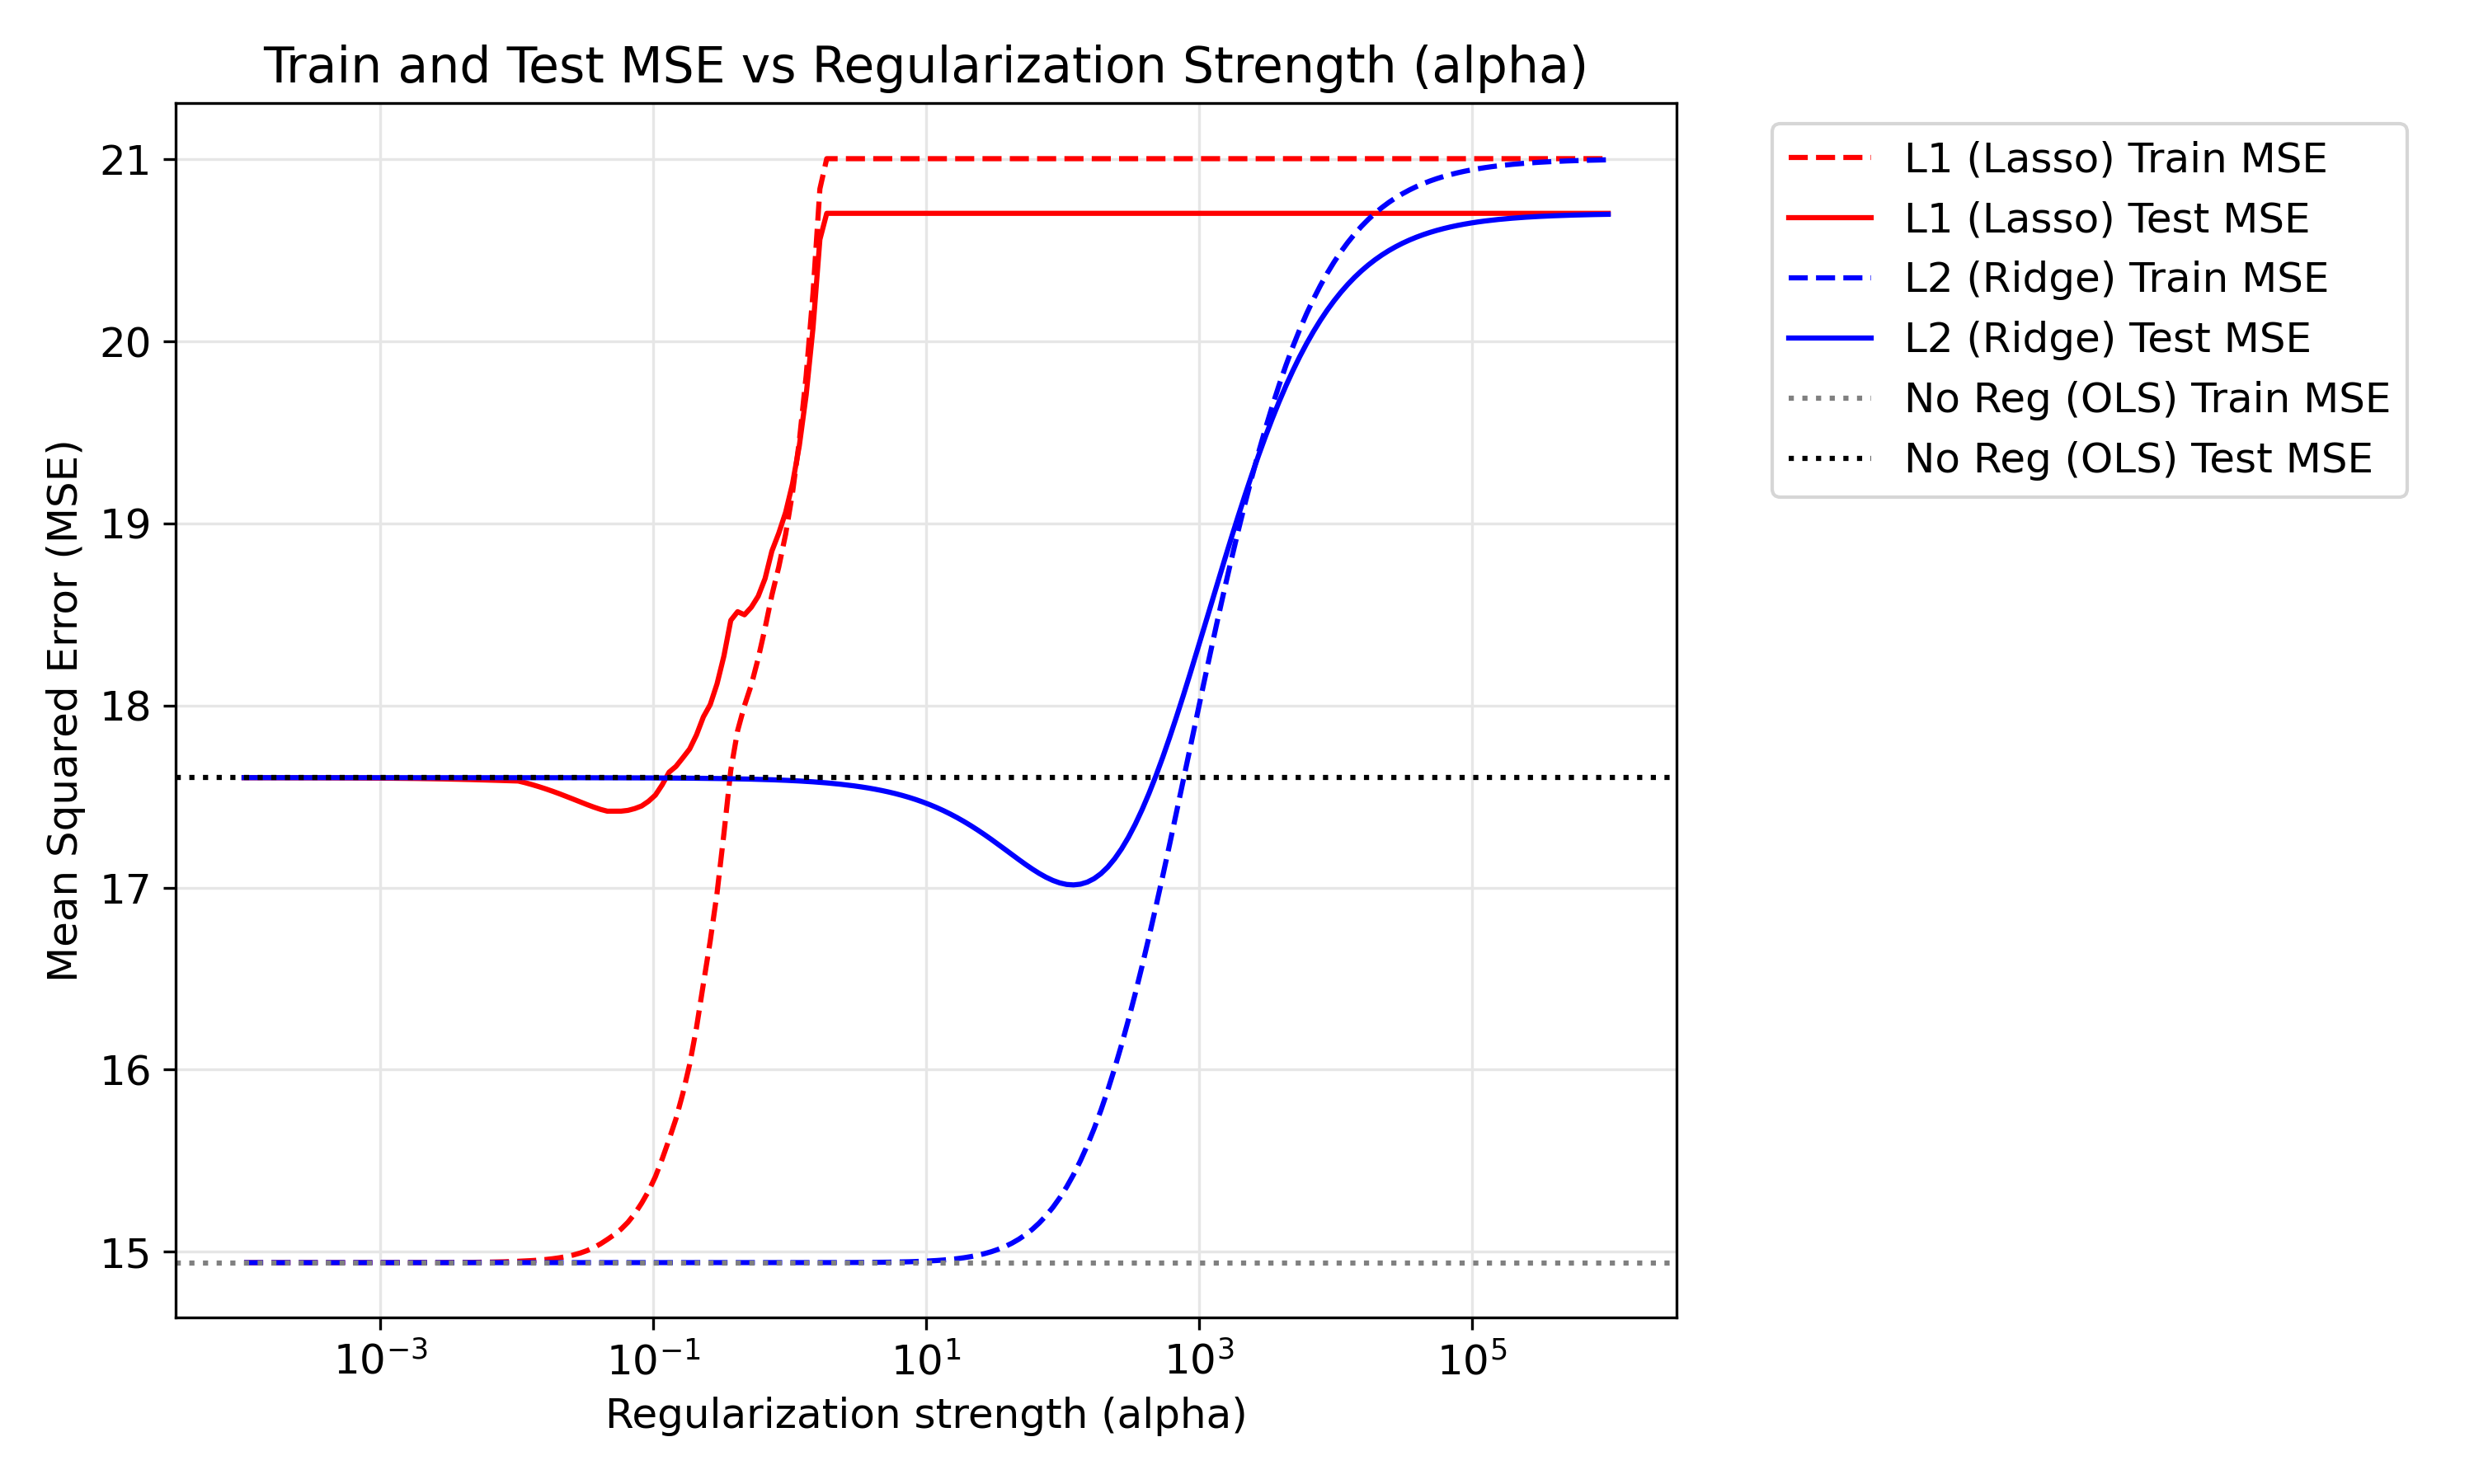
\includegraphics[width=0.7\textwidth]{problem1/plots/mse_comparison.png}
    \caption{正則化強度 $\alpha$ に対する Train/Test MSE の比較}
    \label{fig:mse_comparison}
\end{figure}

\begin{itemize}
    \item OLS: Train 14.9390, Test 17.6037
    \item Lasso: 最小 Test 17.4193 ($\alpha \approx 0.052$)
    \item Ridge: 最小 Test 17.0144 ($\alpha \approx 120.3$)
\end{itemize}
\end{proofbox}

\subsection*{1.2}
\begin{note}
同じく、正則化強度 $\alpha$ を $10^{-4} \sim 10^6$ の範囲で動かし、$10^{-6}$ より大きい重みの数をモデル同士で比較するグラフを作成せよ。
\end{note}
\begin{proofbox}
正則化強度 $\alpha$ に対するアクティブな重み（$|w| > 10^{-6}$）の数を図\ref{fig:weight_comparison}に示す。

\begin{figure}[H]
    \centering
    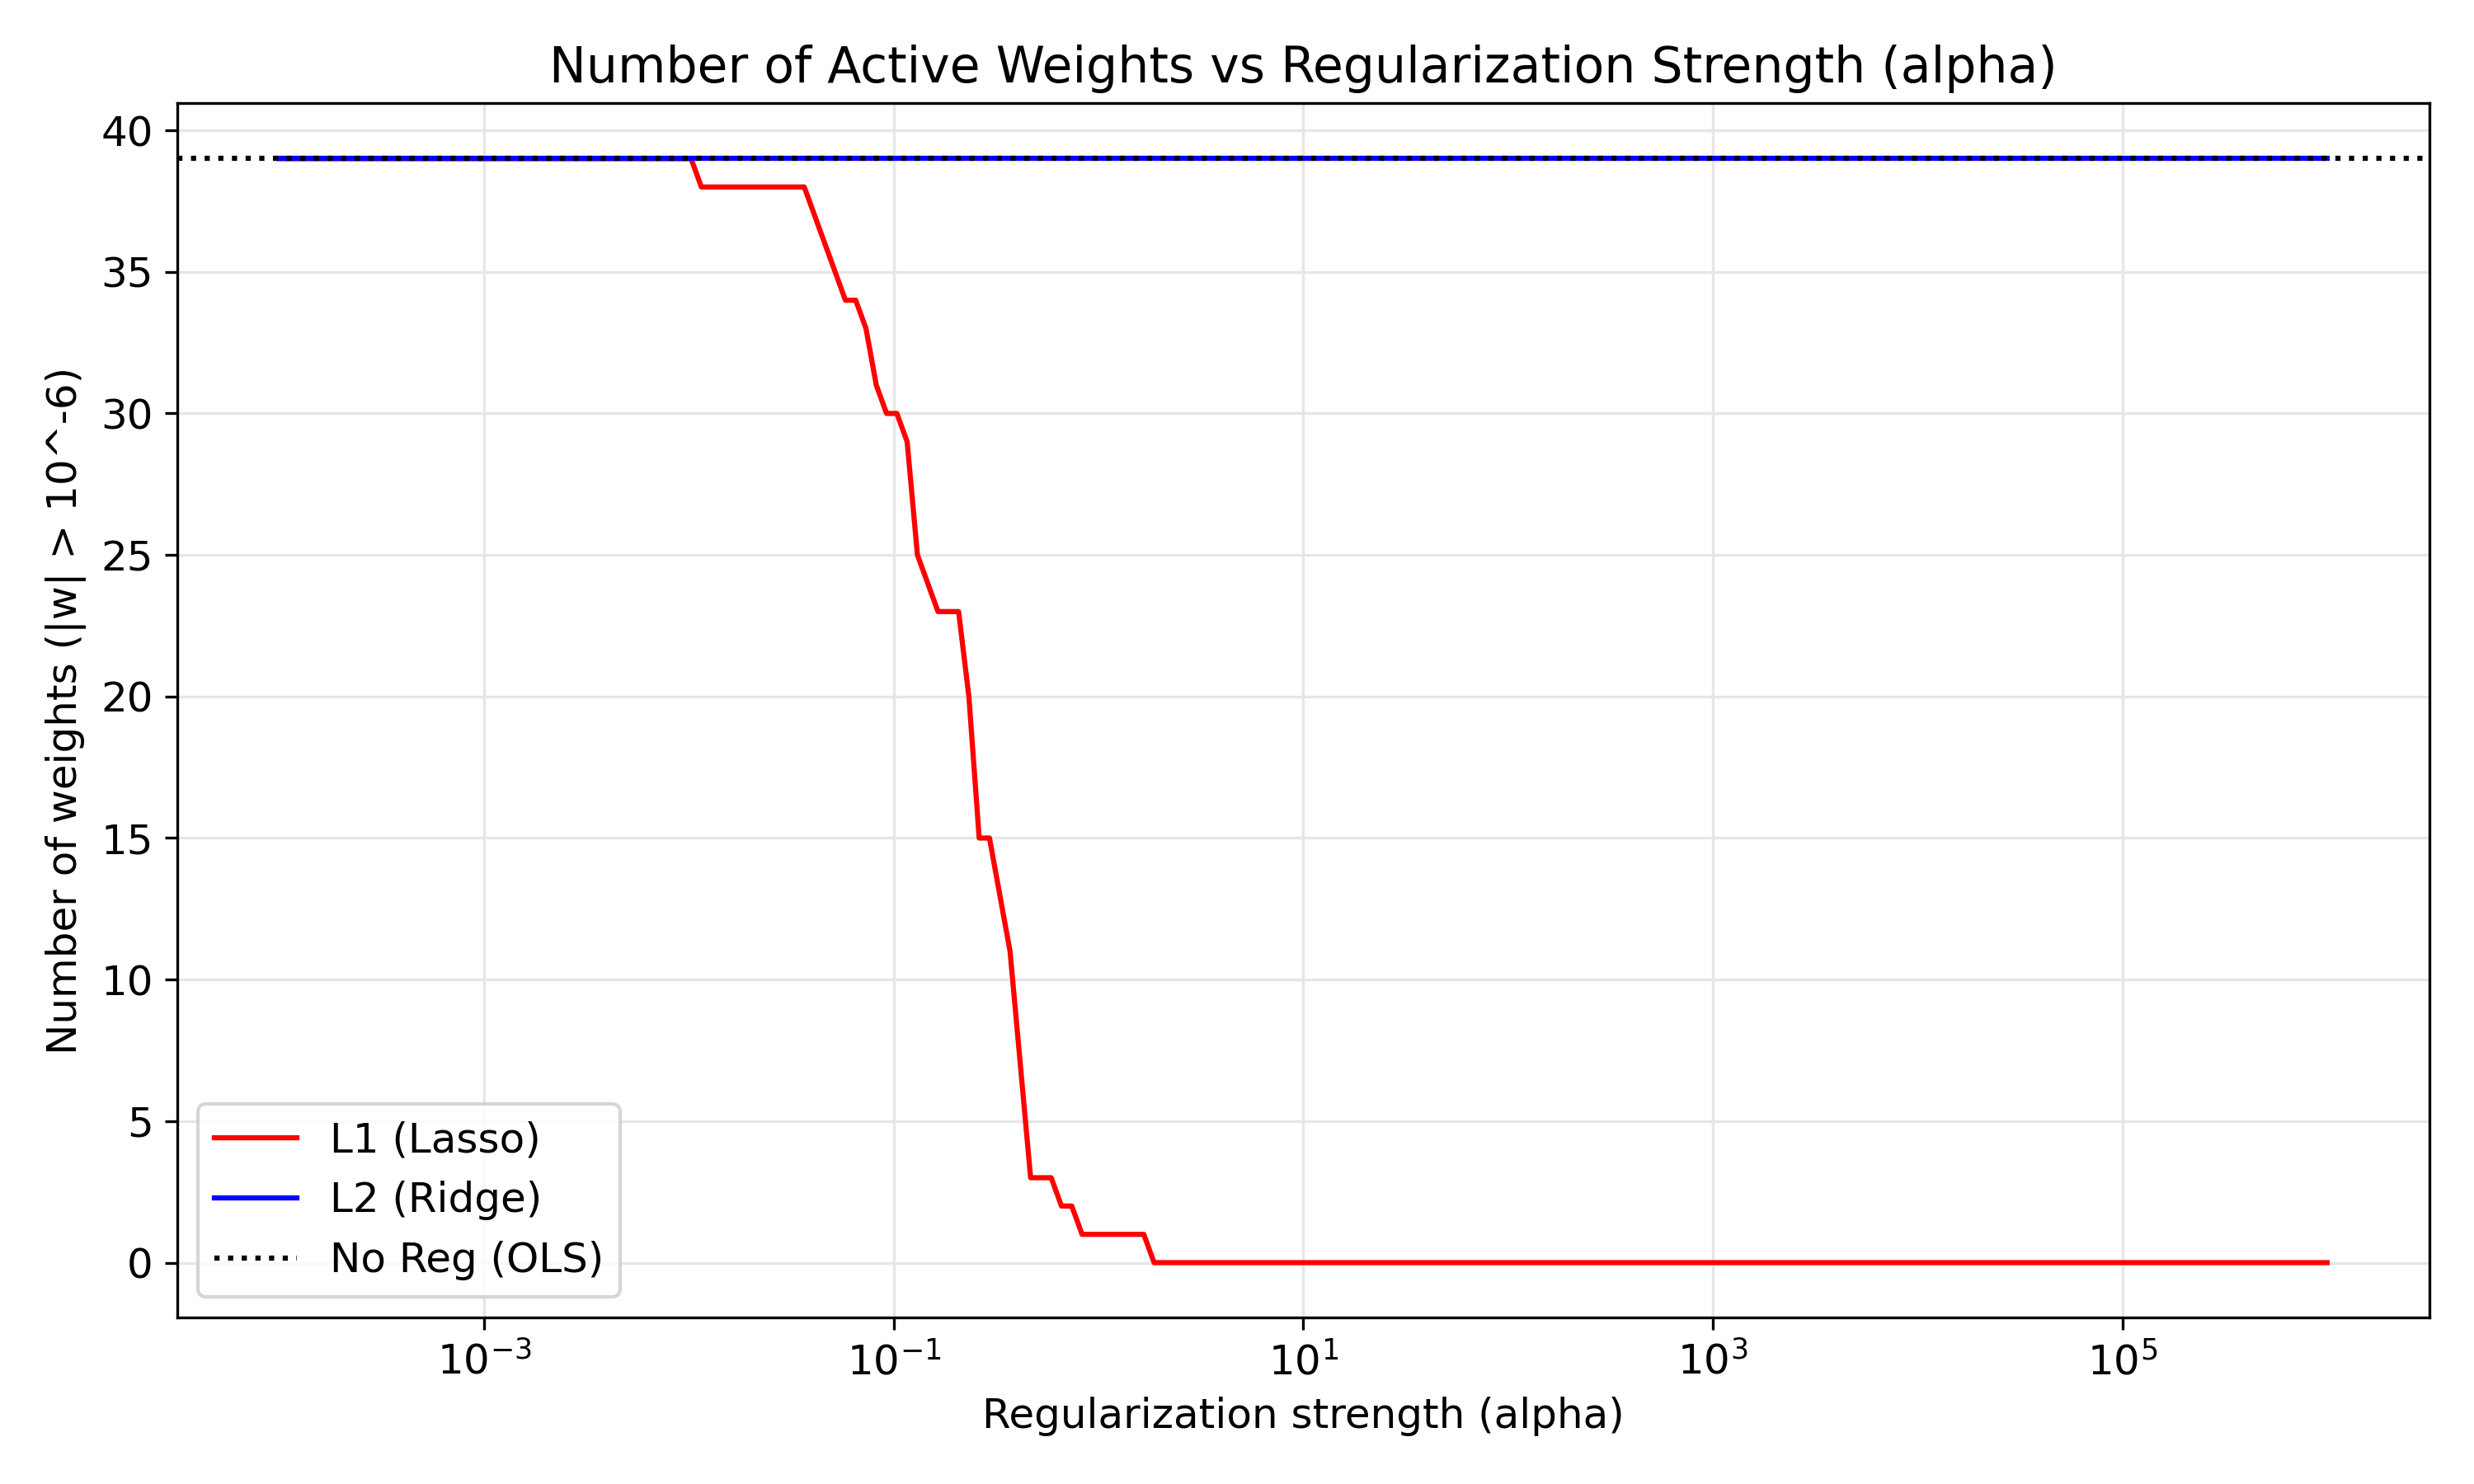
\includegraphics[width=0.7\textwidth]{problem1/plots/weight_comparison.png}
    \caption{正則化強度 $\alpha$ に対するアクティブな重み数の変化}
    \label{fig:weight_comparison}
\end{figure}

Lassoは $\alpha \approx 10^{-2}$ から有効特徴量が急減し、$\alpha \ge 10$ で全て 0 になる。一方、Ridgeはペナルティが平方和であるため重みを完全に 0 にせず、$\alpha = 10^6$ でも39個の特徴量がすべてアクティブな状態を維持している。
\end{proofbox}

\subsection*{1.3}
\begin{note}
上の 2 つの実験で得られた結果について観察し、気付いたことを 3 つ以上挙げよ。考察はここでは書かず次に書くこと。
\end{note}
\begin{proofbox}
実験結果から得られた主な観察は以下の3点である。第1に、適度な正則化強度 $\alpha$ において Test MSE が減少しており、過学習が抑制されている。第2に、本タスクではRidge（Test MSE: 17.01）がLasso（17.42）やOLS（17.60）よりも低いテスト誤差を達成しており、性能面で優位である。第3に、Lassoは $\alpha \approx 0.05$ の段階で一部の重みを完全に 0 にして特徴量選択を行っているのに対し、Ridgeは $\alpha = 10^6$ に至るまで全特徴量の重みを非ゼロに保ちながら滑らかに縮小させている。
\end{proofbox}

\subsection*{1.4}
\begin{note}
L1 では重みが 0 になる特徴量が多く現れることが予想される。その理由を説明せよ。また、観察した他の事項についても、説明がつけば考察せよ。
\end{note}
\begin{proofbox}
L1正則化（Lasso）の目的関数に課される制約 $\sum |w_j| \le C$ は、パラメータ空間において各座標軸上に尖点（角）を持つダイヤモンド型の領域となる。二乗誤差の等高線（楕円）がこの制約領域と接する最適解は、角で接しやすいため一部のパラメータが完全に 0 になりやすい（スパース性）。対して、L2正則化の制約 $\sum w_j^2 \le C$ は滑らかな超球面であるため、パラメータは縮小するものの完全に 0 にはなりにくい。

本実験のLassoで重みが 0 になった特徴量には \texttt{Fedu} や \texttt{Walc} などが含まれており、これらは他の相関が高い特徴量（\texttt{Medu} や \texttt{Dalc} など）に対して情報が冗長であったと考えられる。また、LassoよりもRidgeの精度が高かった点から、本データセットの期末成績は少数の要因のみに支配されているのではなく、多くの家庭環境や学習状況が複合的に寄与している「密（dense）」な関係にあると推察される。
\end{proofbox}

\subsection*{1.5}
\begin{note}
L1、L2 以外の正則化項を 1 つ提案せよ。その正則化項を用いることでどのような効果が期待できるか説明せよ。
\end{note}
\begin{proofbox}
L1とL2正則化のハイブリッドである Elastic Net を提案する。目的関数は以下のように定義される。
\begin{equation}
E_{\text{ElasticNet}}(\bm{w}) = \frac{1}{2M} \|\bm{y} - X\bm{w}\|_2^2 + \alpha \left( \rho \sum_{j=1}^N |w_j| + \frac{1-\rho}{2} \sum_{j=1}^N w_j^2 \right)
\end{equation}
ここで $\rho \in [0, 1]$ はL1とL2の混合比率を表す。これにより期待できる効果は主に2点ある。第1に、相関の強い特徴量グループ（多重共線性）がある場合にLassoのように1つだけをランダムに選ぶのではなく、グループ全体を縮小しつつ選択する「グループ選択効果」が得られる。第2に、特徴量数 $p$ がサンプル数 $n$ より大きい場合でも、Lassoの制約（最大 $n$ 個しか選択できない）を超えてスパースな選択が可能になり、解釈性と予測精度の両立が期待できる。
\end{proofbox}


\section{決定木の比較}
\begin{note}
上と同じ DATASET のデータで、今度は決定木回帰を行う。学習の際はデータを $\text{Train}:\text{Test}= 8 : 2$ で分割すること。
\end{note}

\subsection*{2.1}
\begin{note}
データに対し、決定木、Bagging、Random Forest の 3 種類で決定木回帰を行う。分割の仕方を変えて決定木回帰を 100 回行い、Test MSE をモデル同士で比較する箱ひげ図を作成せよ。ただし、決定木の深さに制限は設けず、Bagging と Random Forest のアンサンブルに使う決定木の本数は 50 とし、Random Forest の $\text{max\_features}=0.6$ とせよ。また、データの前処理についても明記せよ。
\end{note}
\begin{proofbox}
One-Hot化と標準化の前処理の後、Train:Test=8:2へのランダム分割を100回行い、単一決定木、Bagging ($B=50$)、Random Forest ($B=50$, $\text{max\_features}=0.6$) の各モデルで Test MSE の分布を比較した。結果を図\ref{fig:boxplot_comparison}に示す。

\begin{figure}[H]
    \centering
    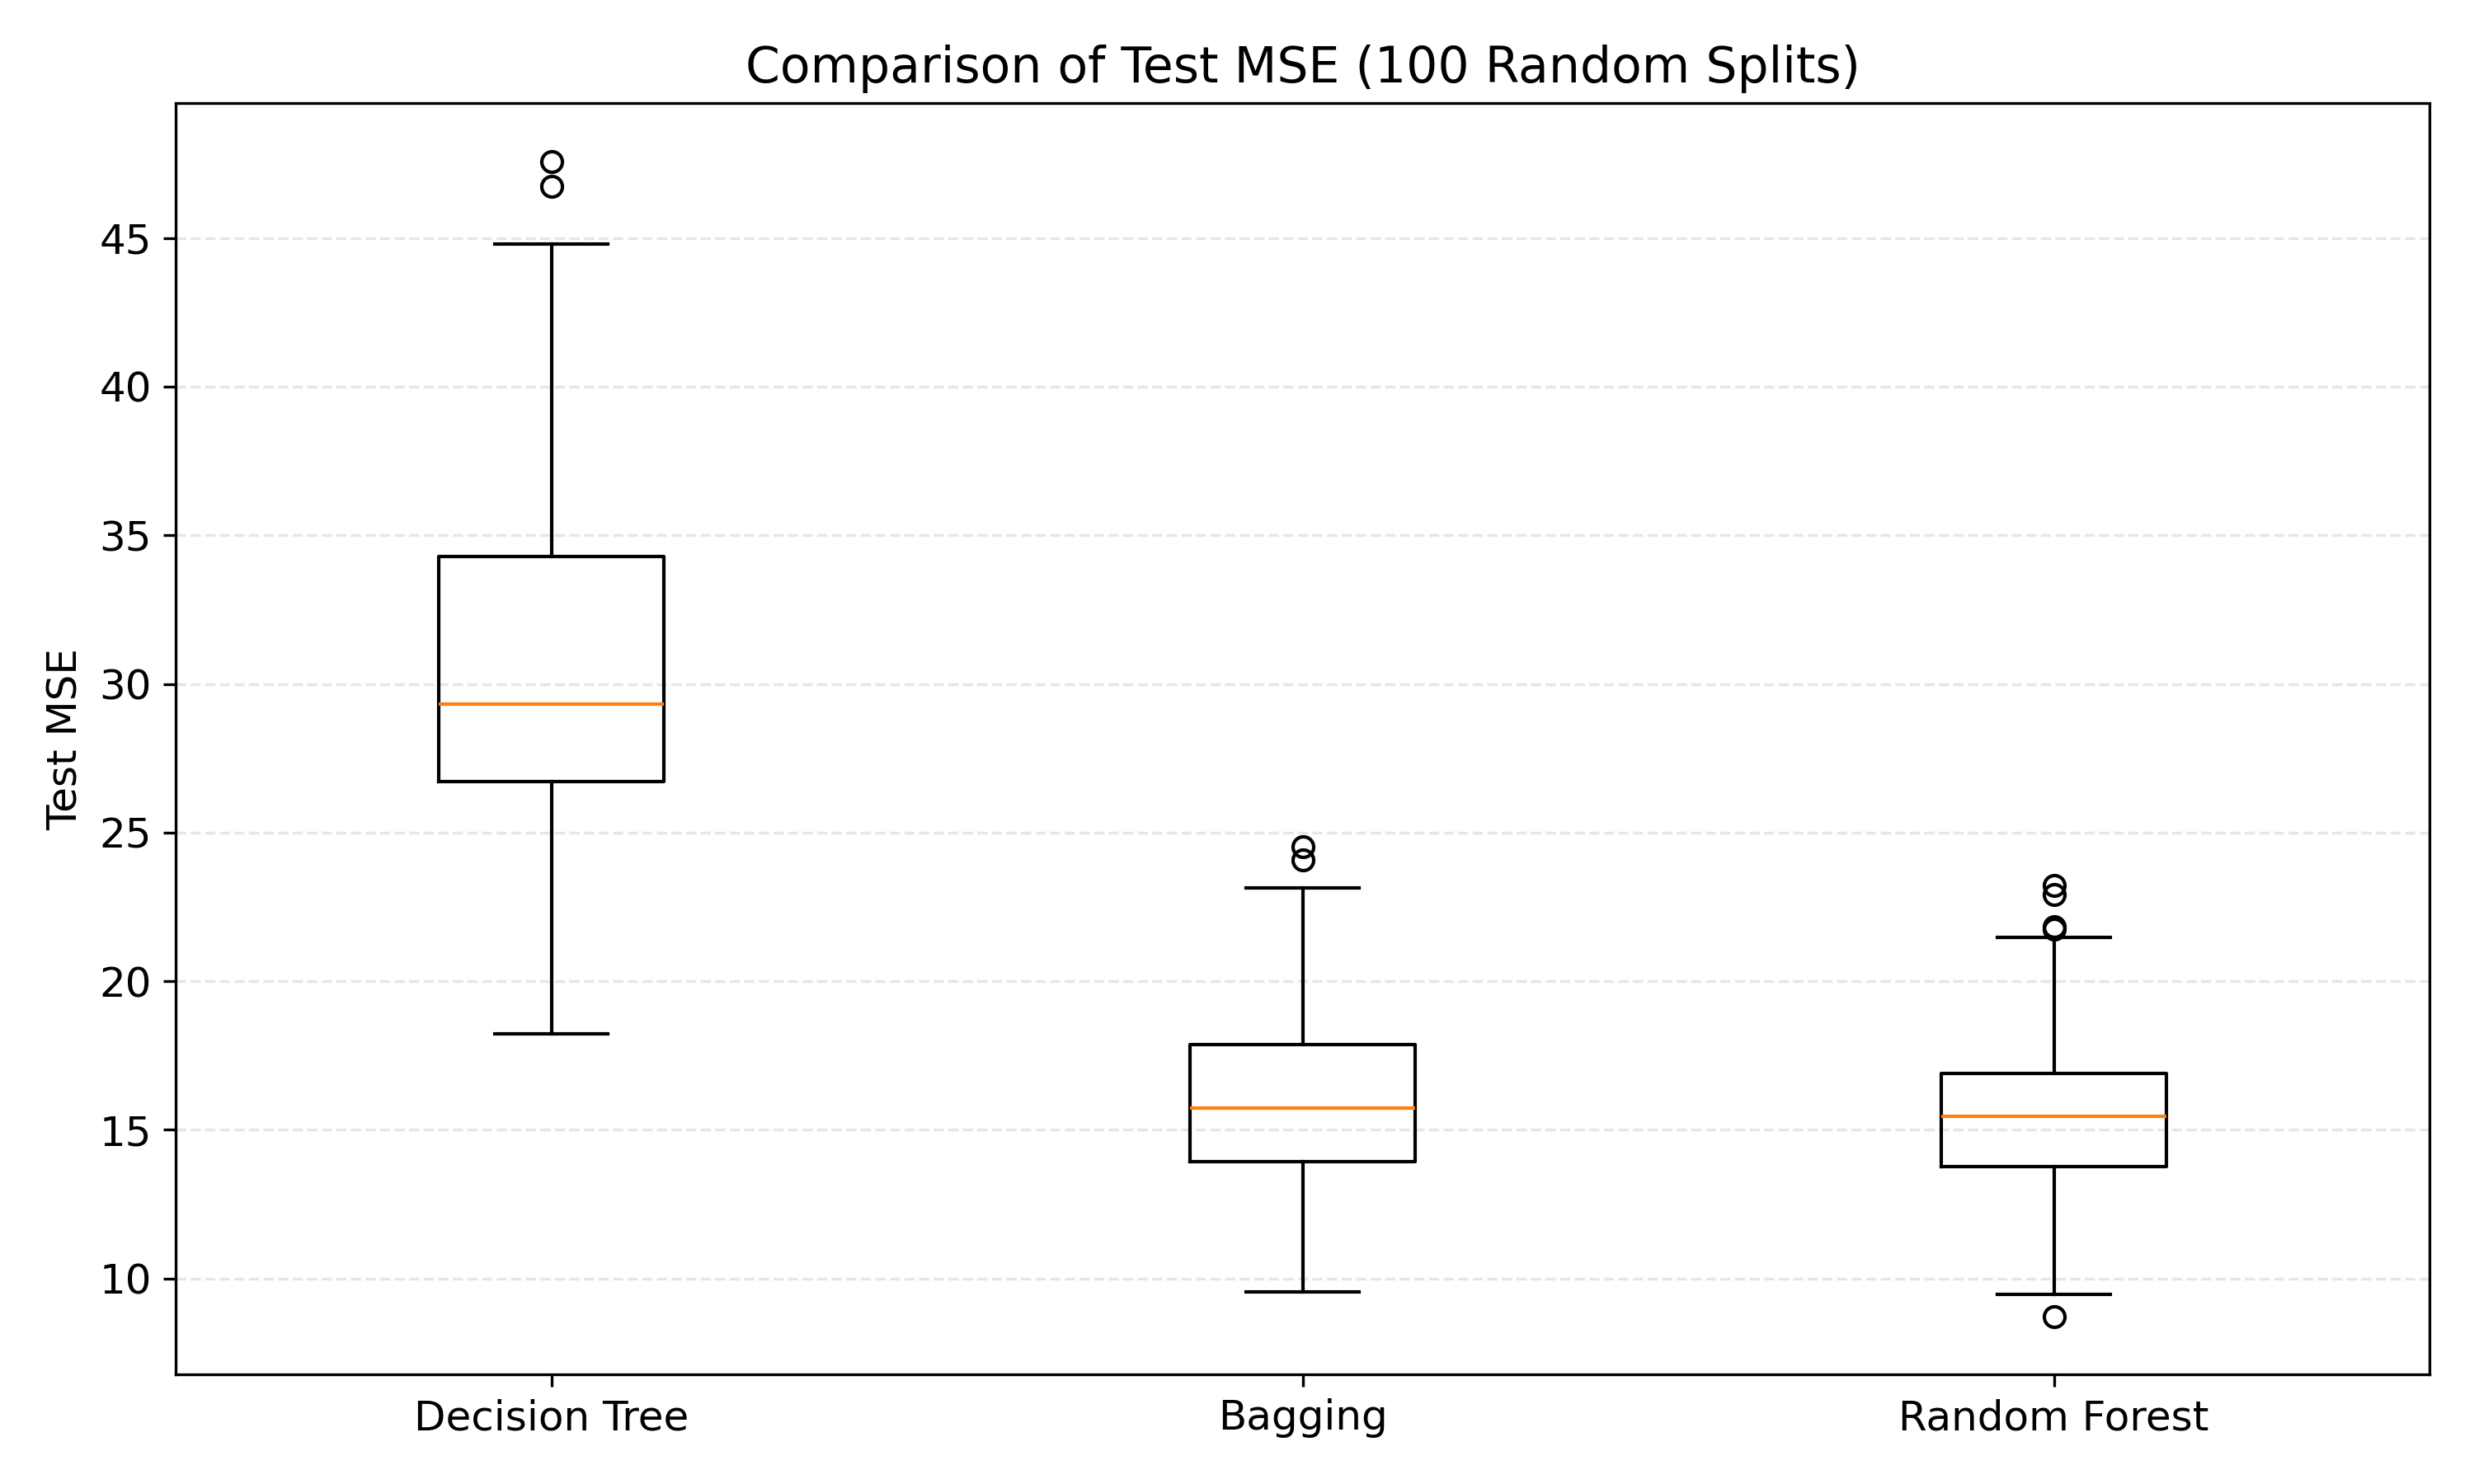
\includegraphics[width=0.7\textwidth]{problem2/plots/boxplot_comparison.png}
    \caption{100回のランダム分割における Test MSE の分布比較}
    \label{fig:boxplot_comparison}
\end{figure}

100回試行の平均 Test MSE は以下の通りであった。
\begin{itemize}
    \item 単一決定木: 30.5632
    \item Bagging: 15.9301
    \item Random Forest: 15.5558
\end{itemize}
\end{proofbox}

\subsection*{2.2}
\begin{note}
次に、データの分割を固定した上で Bagging と Random Forest による決定木回帰を行う。アンサンブルに使う決定木の本数 $B$ を $2^0 \sim 2^8$ まで変化させる。各 $B$ に対して乱数シードを変えながら決定木回帰を 50 回行い、固定したある 1 点のテストデータ $x_i$ に対する予測値 $\hat{f}(x_i)$ の分散 $V[\hat{f}(x_i)]$ を求め、その値を $B$ の関数として $\log-\log$ グラフを作成せよ。ただし、決定木の深さに制限は設けず、Random Forest の $\text{max\_features}=0.6$ とせよ。
\end{note}
\begin{proofbox}
データ分割を固定し、テストデータの最初の1点 $x_i$ に対する予測分散 $V[\hat{f}(x_i)]$ のアンサンブル数 $B \in \{2^0 \dots 2^8\}$ に対する変化をシミュレーションした。訓練データのサンプリングばらつき（周辺分散）を評価するため、プールから毎回異なるシードで80\%を抽出して50回モデルを学習させた。得られた $B$ と分散の $\log-\log$ プロットを図\ref{fig:variance_loglog}に示す。

\begin{figure}[H]
    \centering
    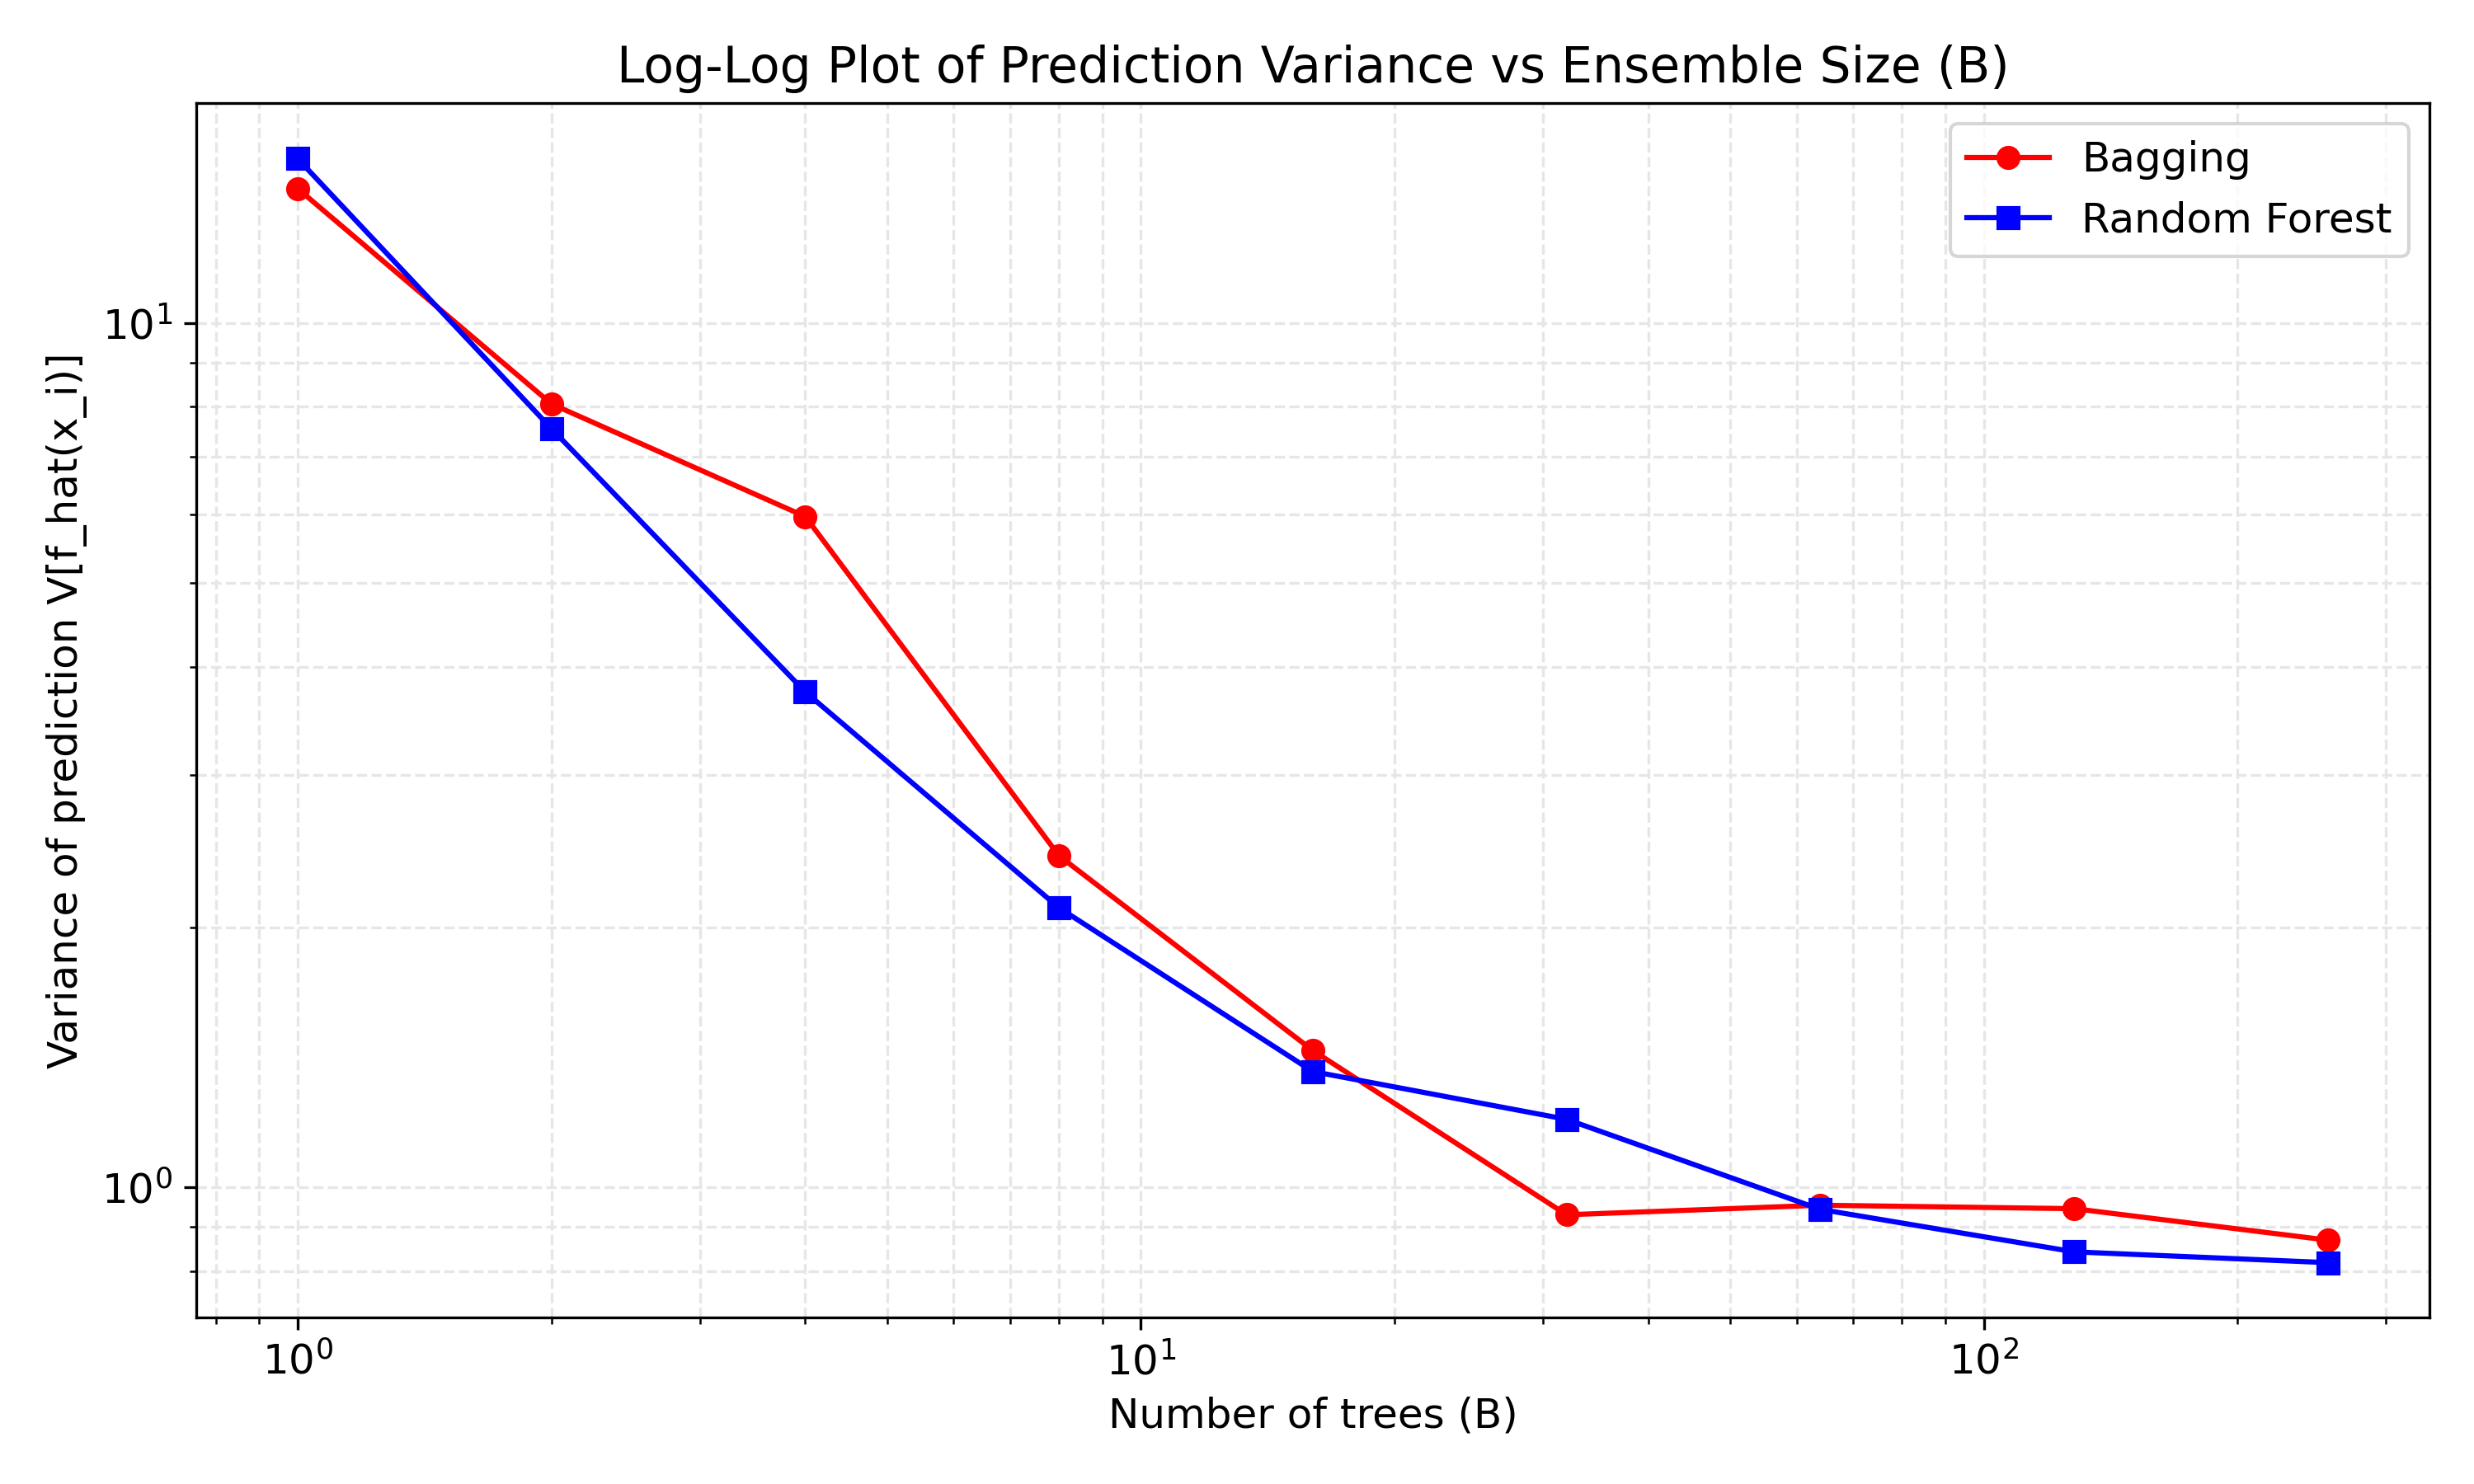
\includegraphics[width=0.7\textwidth]{problem2/plots/variance_loglog.png}
    \caption{アンサンブル数 $B$ に対する予測値の周辺分散の $\log-\log$ 変化}
    \label{fig:variance_loglog}
\end{figure}
\end{proofbox}

\subsection*{2.3}
\begin{note}
上の 2 つの実験で得られた結果について観察し、気付いたことを 3 つ以上挙げよ。考察はここでは書かず次に書くこと。
\end{note}
\begin{proofbox}
実験結果より以下のことが観察される。第1に、単一決定木に比べてBaggingおよびRandom ForestはテストMSEが約半分に激減しており、アンサンブルの効果が極めて大きい。第2に、木の本数 $B=1$ においては、単一のRF（15.48）のほうが単一のBagging（14.30）よりも予測分散が大きくなっている。これは特徴量のサブサンプリングがモデル構築にさらなるランダム性を与えるためである。（※B=1における予測分散はてっきりBaggingのほうが大きいと思い込んでいたが、特徴量制限のランダム性が加わる分RFのほうがばらつくのは後から考えれば当然だった。）第3に、アンサンブル数 $B$ の増加に伴い周辺分散は減少するが、ある程度（$B \ge 32$ 付近）から頭打ちになって下限（床値）に張り付く。この下限はRF（約0.82）のほうがBagging（約0.87）よりも低い。
\end{proofbox}

\subsection*{2.4}
\begin{note}
決定木に比べ Bagging や Random Forest は Test MSE が小さくなることが予想される。その理由を説明せよ。また、上の $\log-\log$ グラフでは Bagging よりも Random Forest の方が直線に近くなることが期待される。その理由を説明せよ。さらに、観察した他の事項についても、説明がつけば考察せよ。
\end{note}
\begin{proofbox}
単一の深い決定木は低バイアス・高バリアンスであるため過学習しやすい。BaggingやRFはブートストラップサンプルにより木を並列学習させて平均化する。アンサンブルモデル全体の分散は、個々の木の分散を $\sigma^2$、木同士の相関を $\rho$、本数を $B$ とすると $V[\hat{f}(x)] = \rho\sigma^2 + \frac{1-\rho}{B}\sigma^2$ となる。$B$ の増加により第2項が消去されバリアンスが下がるため、Test MSEが劇的に減少する。

両対数プロットにおいて、木同士が独立（$\rho=0$）なら $\log V \propto -\log B$ の完全な直線（傾き $-1$）になるが、相関 $\rho > 0$ があると極限値 $\rho\sigma^2$ が床となって頭打ちになる。Baggingは全特徴量を使うため木同士の相関 $\rho_{\text{Bagging}}$ が高く、早期に頭打ちになる。一方、RFはノード分割時に特徴量をランダム制限（今回は60\%）するため、木同士の独立性が高まり相関 $\rho_{\text{RF}}$ が著しく低下する。その結果、周辺分散においてRFはより広い範囲で $1/B$ に比例した減少が働き、より直線に近い挙動を示す。

【訓練データを30\%（重複低減）にした追加シミュレーション】
Train = 80\% ではサンプリング元の共通度が高く相関 $\rho$ が非常に大きかったため、訓練データの重複を約9\%まで下げた追加実験（図\ref{fig:variance_loglog_C}）を行った。その結果、アンサンブルによる分散削減が顕著になり、極限の床値においてRF（約1.6）がBagging（約1.8）よりも明確に低い位置へ分離する様子が確認できた。

\begin{figure}[H]
    \centering
    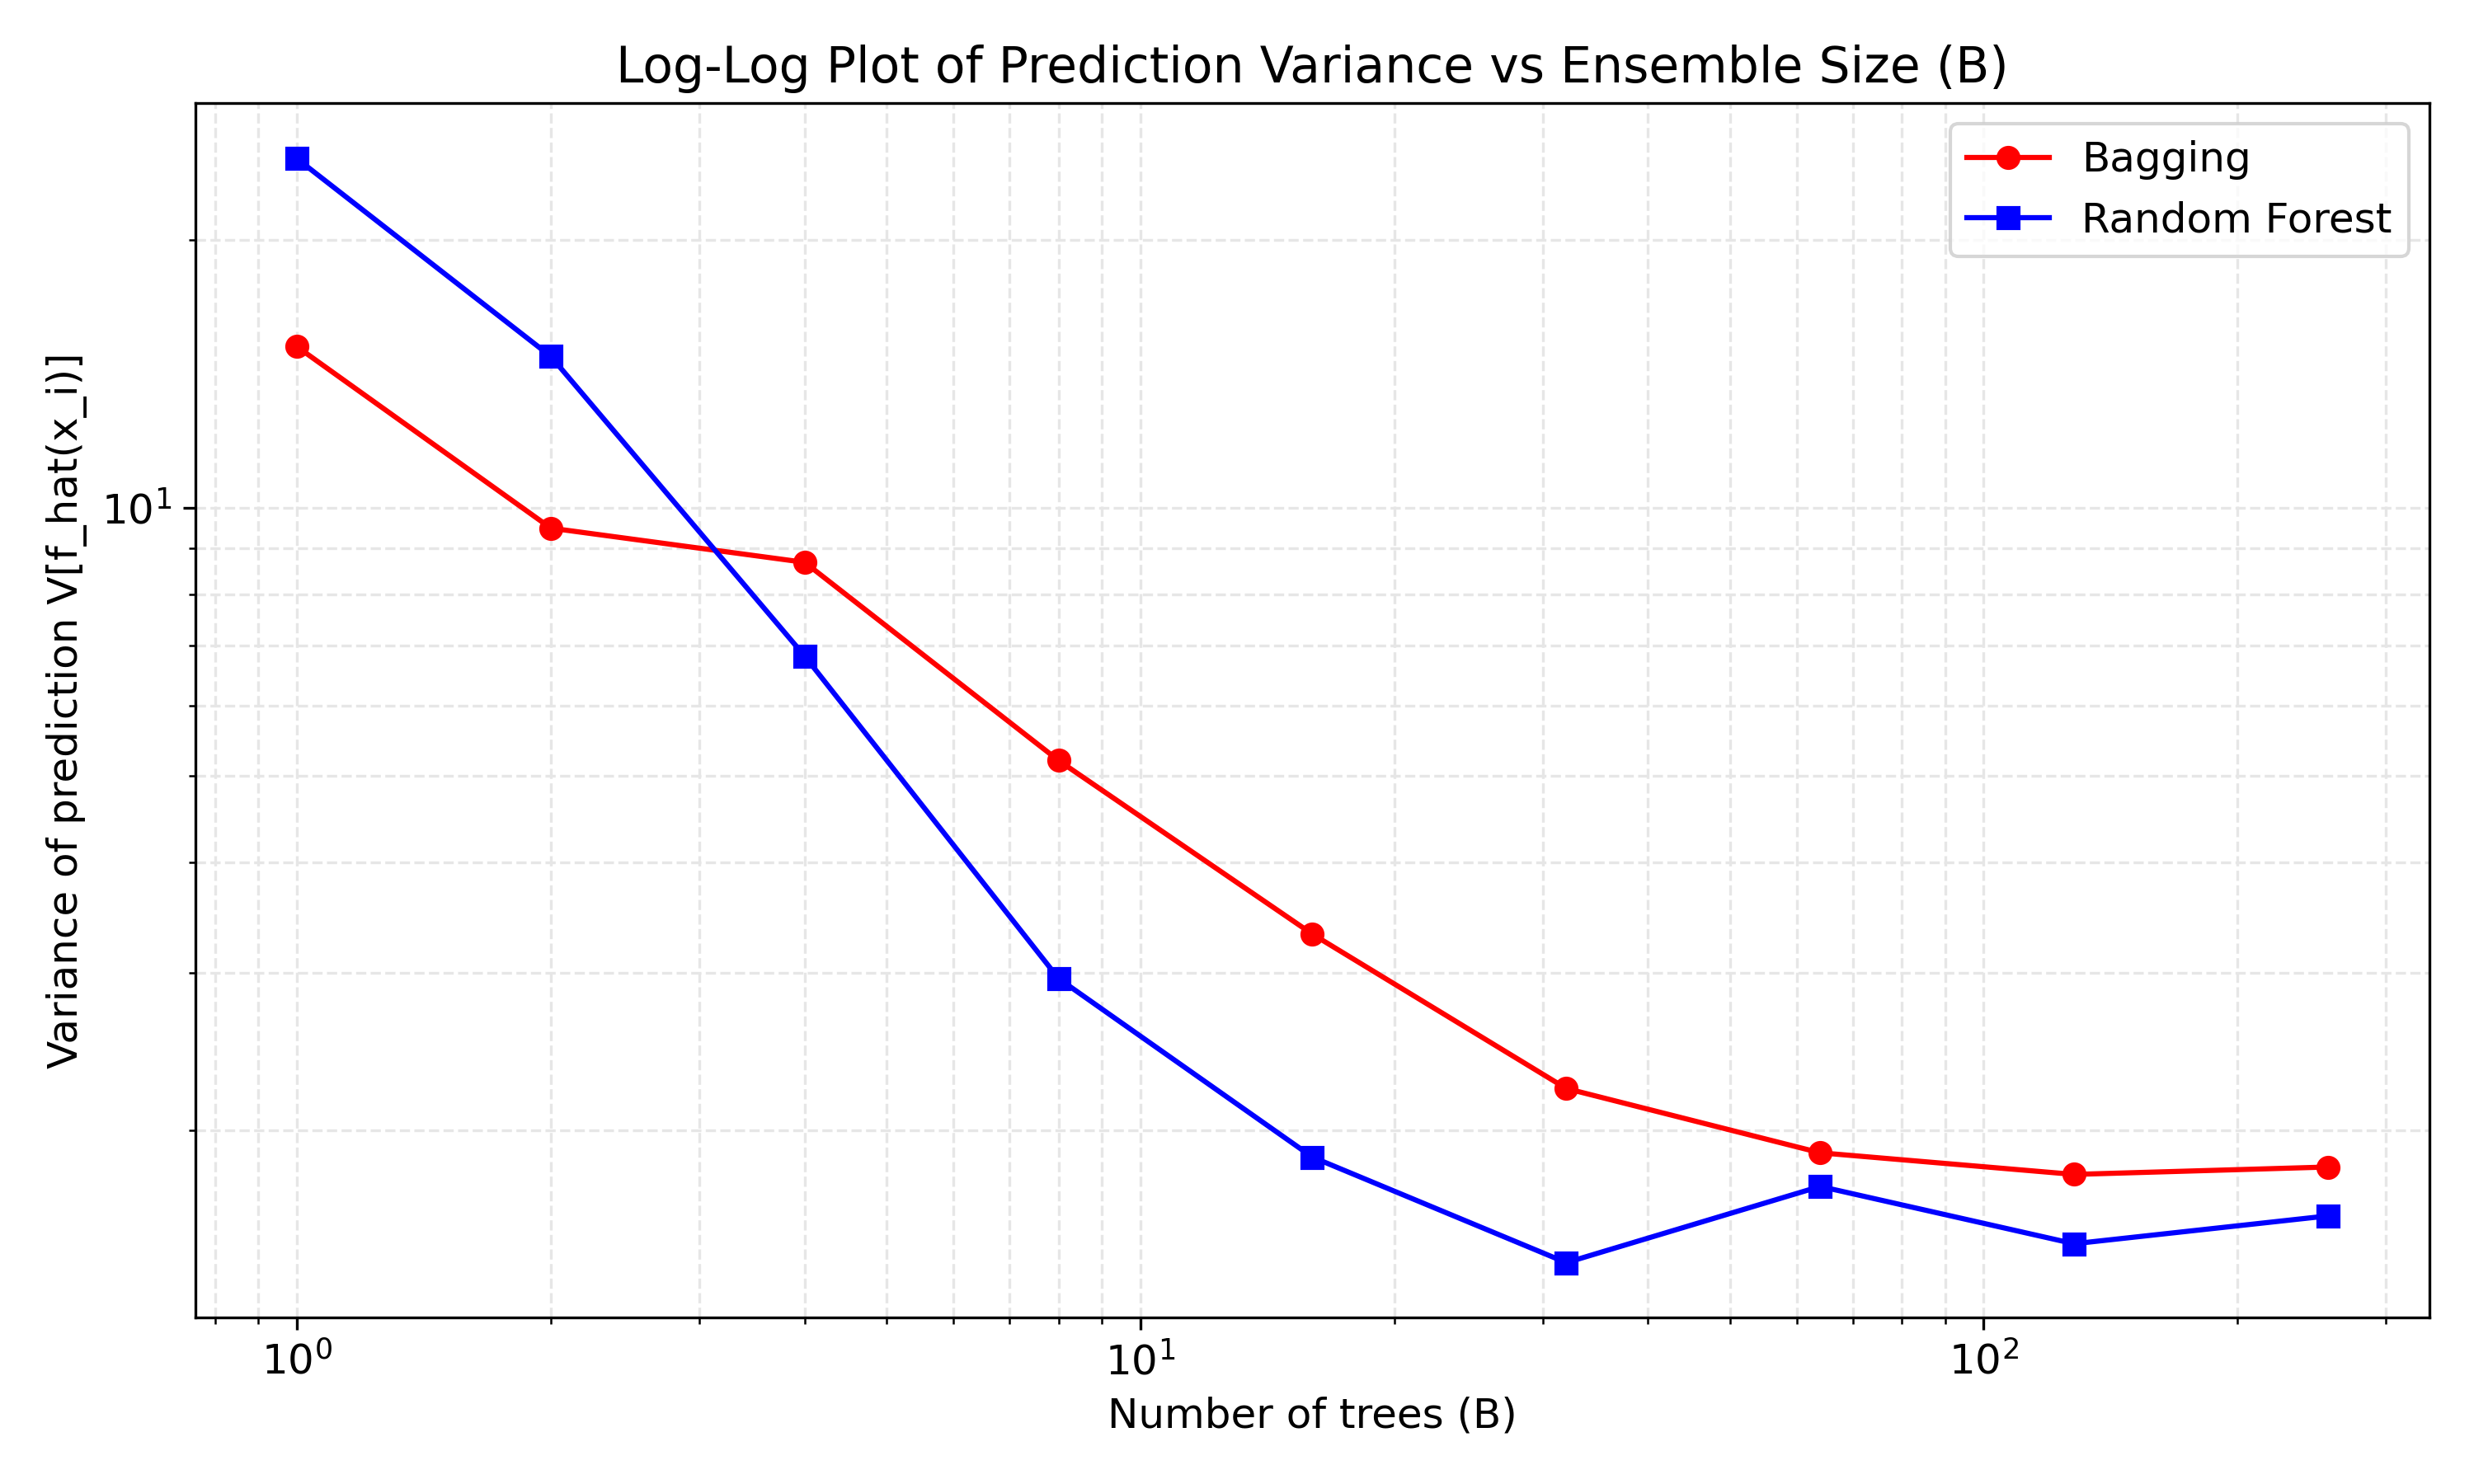
\includegraphics[width=0.7\textwidth]{problem2/plots/variance_loglog_C.png}
    \caption{訓練データ比率30\%における周辺分散の $B$ に対する変化}
    \label{fig:variance_loglog_C}
\end{figure}
\end{proofbox}


\section{Kullback-Leibler 情報量}

\subsection*{3.1}
\begin{note}
情報エントロピー $S(p)$ と KL ダイバージェンス $\text{KL}(p \parallel q)$ の定義を書け。
\end{note}
\begin{proofbox}
確率分布 $p(x)$ のエントロピー $S(p)$ および $p(x)$ と $q(x)$ の間のKLダイバージェンス $\text{KL}(p \parallel q)$ は以下のように定義される。
\begin{equation}
S(p) = - \sum_{x} p(x) \log p(x), \quad \text{KL}(p \parallel q) = \sum_{x} p(x) \log \frac{p(x)}{q(x)}
\end{equation}
\end{proofbox}

\subsection*{3.2}
\begin{note}
KL ダイバージェンス $\text{KL}(q \parallel p)$ の $p(x)$ にボルツマン分布 $p(x) = \frac{\exp(-\beta E(x))}{Z}$ を代入し、自由エネルギーの差分の形に整理せよ。
\end{note}
\begin{proofbox}
KLダイバージェンスの定義にボルツマン分布 $p(x) = \frac{\exp(-\beta E(x))}{Z}$ を代入する。
\begin{align}
\text{KL}(q \parallel p) &= \sum_{x} q(x) \log q(x) - \sum_{x} q(x) \log p(x) \notag \\
&= -S(q) + \beta \sum_{x} q(x) E(x) + \log Z \sum_{x} q(x) \notag \\
&= \beta \langle E \rangle_q - S(q) + \log Z
\end{align}
両辺を $\beta$ で割り、ヘルムホルツ自由エネルギー $F(p) = -\frac{1}{\beta}\log Z$ および変分自由エネルギー $F(q) = \langle E \rangle_q - \frac{1}{\beta}S(q)$ を用いると、自由エネルギーの差分の形で整理される。
\begin{equation}
\frac{1}{\beta} \text{KL}(q \parallel p) = F(q) - F(p)
\end{equation}
\end{proofbox}

\subsection*{3.3}
\begin{note}
KL ダイバージェンスが非負であることを示せ。
\end{note}
\begin{proofbox}
対数関数 $\log t$ は上に凸な関数であるため、確率重み $p(x)$ に対するイェンセンの不等式を用いると以下が成り立つ。
\begin{align}
-\text{KL}(p \parallel q) = \sum_{x} p(x) \log \frac{q(x)}{p(x)} \le \log \left( \sum_{x} q(x) \right) = \log 1 = 0
\end{align}
したがって $\text{KL}(p \parallel q) \ge 0$ が示された。等号成立は $\frac{q(x)}{p(x)} = \text{const}$、すなわち規格化条件より $p(x) = q(x) \ (\forall x)$ のときに限る。
\begin{equation}
\text{KL}(p \parallel q) \ge 0 \quad (\text{等号は } p = q \text{ のときのみ})
\end{equation}
\end{proofbox}

\subsection*{3.4}
\begin{note}
以上の結果から、KL ダイバージェンスが統計力学的にどう解釈できるか説明せよ。
\end{note}
\begin{proofbox}
3.2節および3.3節より $F(q) \ge F(p)$ （等号は $q=p$ のみ）が成り立つ。これは、一定温度 $T$ の熱浴と接する系において、自由エネルギー $F(q)$ を最小にする唯一の確率分布が熱平衡状態のボルツマン分布 $p$ であるという「自由エネルギー最小化の原理」を表している。また、物理的な自由エネルギーの差 $F(q) - F(p)$ は非平衡状態 $q$ から平衡状態 $p$ に遷移する際にとりうる最大仕事（あるいは散逸する自由エネルギー）に相当するため、KLダイバージェンス $\text{KL}(q \parallel p)$ は単なる情報論的乖離度にとどまらず、系の「熱力学的非平衡度（散逸損失）」を測る物理量として解釈できる。
\end{proofbox}


\section{線形回帰の理論誤差}
\begin{note}
出力データ $\bm{y} \in \mathbb{R}^n$ が $\bm{y} = X\bm{\beta} + \bm{\epsilon}$ に従って生成されているとする。ただし、$X \in \mathbb{R}^{n \times p}$, $\bm{\beta} \in \mathbb{R}^{p \times 1}$, $\bm{\epsilon} \in \mathbb{R}^{n \times 1}$ であり、意味としては $X$ が入力データ、$\bm{\beta}$ がパラメータ、$\bm{\epsilon}$ がノイズに対応する。$X_{i,:} \sim N(0, I_p)$、$\bm{\epsilon} \sim N(0, \sigma^2 I_n)$ とする。
\end{note}

\subsection*{4.1}
\begin{note}
重みの推定量として、最小二乗推定量
\begin{equation*}
\hat{\bm{\beta}} = \arg\min_{\bm{\beta}} \|\bm{y} - X\bm{\beta}\|^2
\end{equation*}
を用いる。観測データ $\bm{y}$ と特徴量データ $X$ が与えられたとき、$\hat{\bm{\beta}}$ を求めよ。必要に応じて擬似逆行列を用いて良い。
\end{note}
\begin{proofbox}
目的関数 $L(\bm{\beta}) = \|\bm{y} - X\bm{\beta}\|^2$ の $\bm{\beta}$ に関する微分を $\bm{0}$ と置くことで、正規方程式 $X^T X \bm{\beta} = X^T \bm{y}$ を得る。
Moore-Penrose 擬似逆行列 $X^+$ を用いると、最小二乗（または最小ノルム）推定量は一意に $\hat{\bm{\beta}} = X^+ \bm{y}$ と求まる。
ここで $X^+$ は以下の通りである。
\begin{equation}
X^+ = \begin{cases} (X^T X)^{-1} X^T & (n \ge p) \\ X^T (X X^T)^{-1} & (n < p) \end{cases}
\end{equation}
\end{proofbox}

\subsection*{4.2}
\begin{note}
推定量 $\hat{\bm{\beta}}$ の $\bm{\epsilon}$ についての期待値 $E[\hat{\bm{\beta}}]$ と共分散行列 $\text{Cov}[\hat{\bm{\beta}}]$ を求めよ。
\end{note}
\begin{proofbox}
データ生成プロセス $\bm{y} = X\bm{\beta} + \bm{\epsilon}$ （$E[\bm{\epsilon}] = \bm{0}$, $\text{Cov}[\bm{\epsilon}] = \sigma^2 I_n$）に対し、推定量 $\hat{\bm{\beta}} = X^+ \bm{y}$ の期待値と共分散行列は以下のように計算される。

\paragraph{1. 期待値 $E[\hat{\bm{\beta}}]$}
$E[\hat{\bm{\beta}}] = X^+ X \bm{\beta}$。
\begin{itemize}
    \item $n \ge p$ のとき: $X^+ X = I_p$ より $E[\hat{\bm{\beta}}] = \bm{\beta}$ （不偏推定量）。
    \item $n < p$ のとき: $X^+ X = X^T (X X^T)^{-1} X = P_X$（$X$ の行空間への直交射影行列）より $E[\hat{\bm{\beta}}] = P_X \bm{\beta}$（バイアスが発生）。
\end{itemize}

\paragraph{2. 共分散行列 $\text{Cov}[\hat{\bm{\beta}}]$}
$\text{Cov}[\hat{\bm{\beta}}] = X^+ \text{Cov}[\bm{y}] (X^+)^T = \sigma^2 X^+ (X^+)^T$。
\begin{itemize}
    \item $n \ge p$ のとき: $\text{Cov}[\hat{\bm{\beta}}] = \sigma^2 (X^T X)^{-1}$。
    \item $n < p$ のとき: $\text{Cov}[\hat{\bm{\beta}}] = \sigma^2 X^T (X X^T)^{-2} X$。
\end{itemize}
\end{proofbox}

\subsection*{4.3}
\begin{note}
テストデータ $\bm{x}_{\text{new}} \in \mathbb{R}^{1 \times p}$ が $N(0, I_p)$ に従って生成されたとする。$\text{Test MSE}$ の期待値を求めよ。ただし、$X$ は残したままで良い。
\end{note}
\begin{proofbox}
テスト入力 $\bm{x}_{\text{new}} \sim N(\bm{0}, I_p)$ とノイズ $\epsilon_{\text{new}} \sim N(0, \sigma^2)$ に対する Test MSE の期待値は、バイアス・バリアンス分解により以下のように書ける。
\begin{align}
E[\text{Test MSE} \mid X] = \sigma^2 + \|\bm{\beta} - E[\hat{\bm{\beta}}]\|^2 + \text{Tr}\left(\text{Cov}[\hat{\bm{\beta}} \mid X]\right)
\end{align}
4.2節の結果を代入して整理する。
\begin{description}
    \item[1. $n \ge p$ の場合]:
    不偏性よりバイアス項は 0 となり、$\text{Cov}[\hat{\bm{\beta}} \mid X] = \sigma^2 (X^T X)^{-1}$ であるから、以下を得る。
    \begin{equation}
    E[\text{Test MSE} \mid X] = \sigma^2 + \sigma^2 \text{Tr}\left( (X^T X)^{-1} \right)
    \end{equation}
    
    \item[2. $n < p$ の場合]:
    バイアス項は $\|\bm{\beta} - P_X \bm{\beta}\|^2 = \bm{\beta}^T (I_p - P_X) \bm{\beta}$ となり、バリアンスのトレースは $\sigma^2 \text{Tr}(X^T(XX^T)^{-2}X) = \sigma^2 \text{Tr}((XX^T)^{-1})$ であるから、以下を得る。（※バリアンス項のトレース計算で、トレースの巡回性 $\text{Tr}(AB)=\text{Tr}(BA)$ を使って $X^T (X X^T)^{-2} X$ が $(X X^T)^{-1}$ に縮約されるのは、線形代数のパズルみたいできれいな変形だと思った。）
    \begin{equation}
    E[\text{Test MSE} \mid X] = \sigma^2 + \bm{\beta}^T \left( I_p - X^T (X X^T)^{-1} X \right) \bm{\beta} + \sigma^2 \text{Tr}\left( (X X^T)^{-1} \right)
    \end{equation}
\end{description}
\end{proofbox}

\subsection*{4.4}
\begin{note}
入力データ数 $n$ を固定した上でパラメータ数 $p$ を動かした時の $\text{Test MSE}$ の変化を観察したい。以下を実装せよ。
\begin{itemize}
    \item $n = 100$ に固定して、$p$ を $10 \sim 400$ の範囲で 5 刻みに動かす
    \item 各 $p$ について 500 回の試行を行う
    \item $\bm{\beta}$ は $N(0, I_p)$ に従うよう生成した後、$\bm{\beta}$ のノルムが $\sqrt{2}$ となるよう規格化し、同じ $p$ では共通とする
    \item 各試行において入力データ $X$ とノイズ $\bm{\epsilon}$ を生成し、推定量 $\hat{\bm{\beta}}$ を計算する
    \item 各試行においてテストデータ $\bm{x}_{\text{new}}$ を 100 個生成し、$\text{Test MSE}$ を計算する
    \item 500 回の試行の平均 $\text{Test MSE}$ を計算する
    \item $\gamma := \frac{p}{n}$ を横軸として平均 $\text{Test MSE}$ をプロットし、グラフを作成する
\end{itemize}
\end{note}
\begin{proofbox}
$n = 100$ に固定し、パラメータ数 $p$ を $10 \sim 400$ の範囲（5刻み）で動かし、各 $p$ で500回の試行を行って Test MSE の挙動をシミュレーションした（スクリプト: \texttt{problem4/simulation.py}）。結果を図\ref{fig:double_descent} に示す。

\begin{figure}[H]
    \centering
    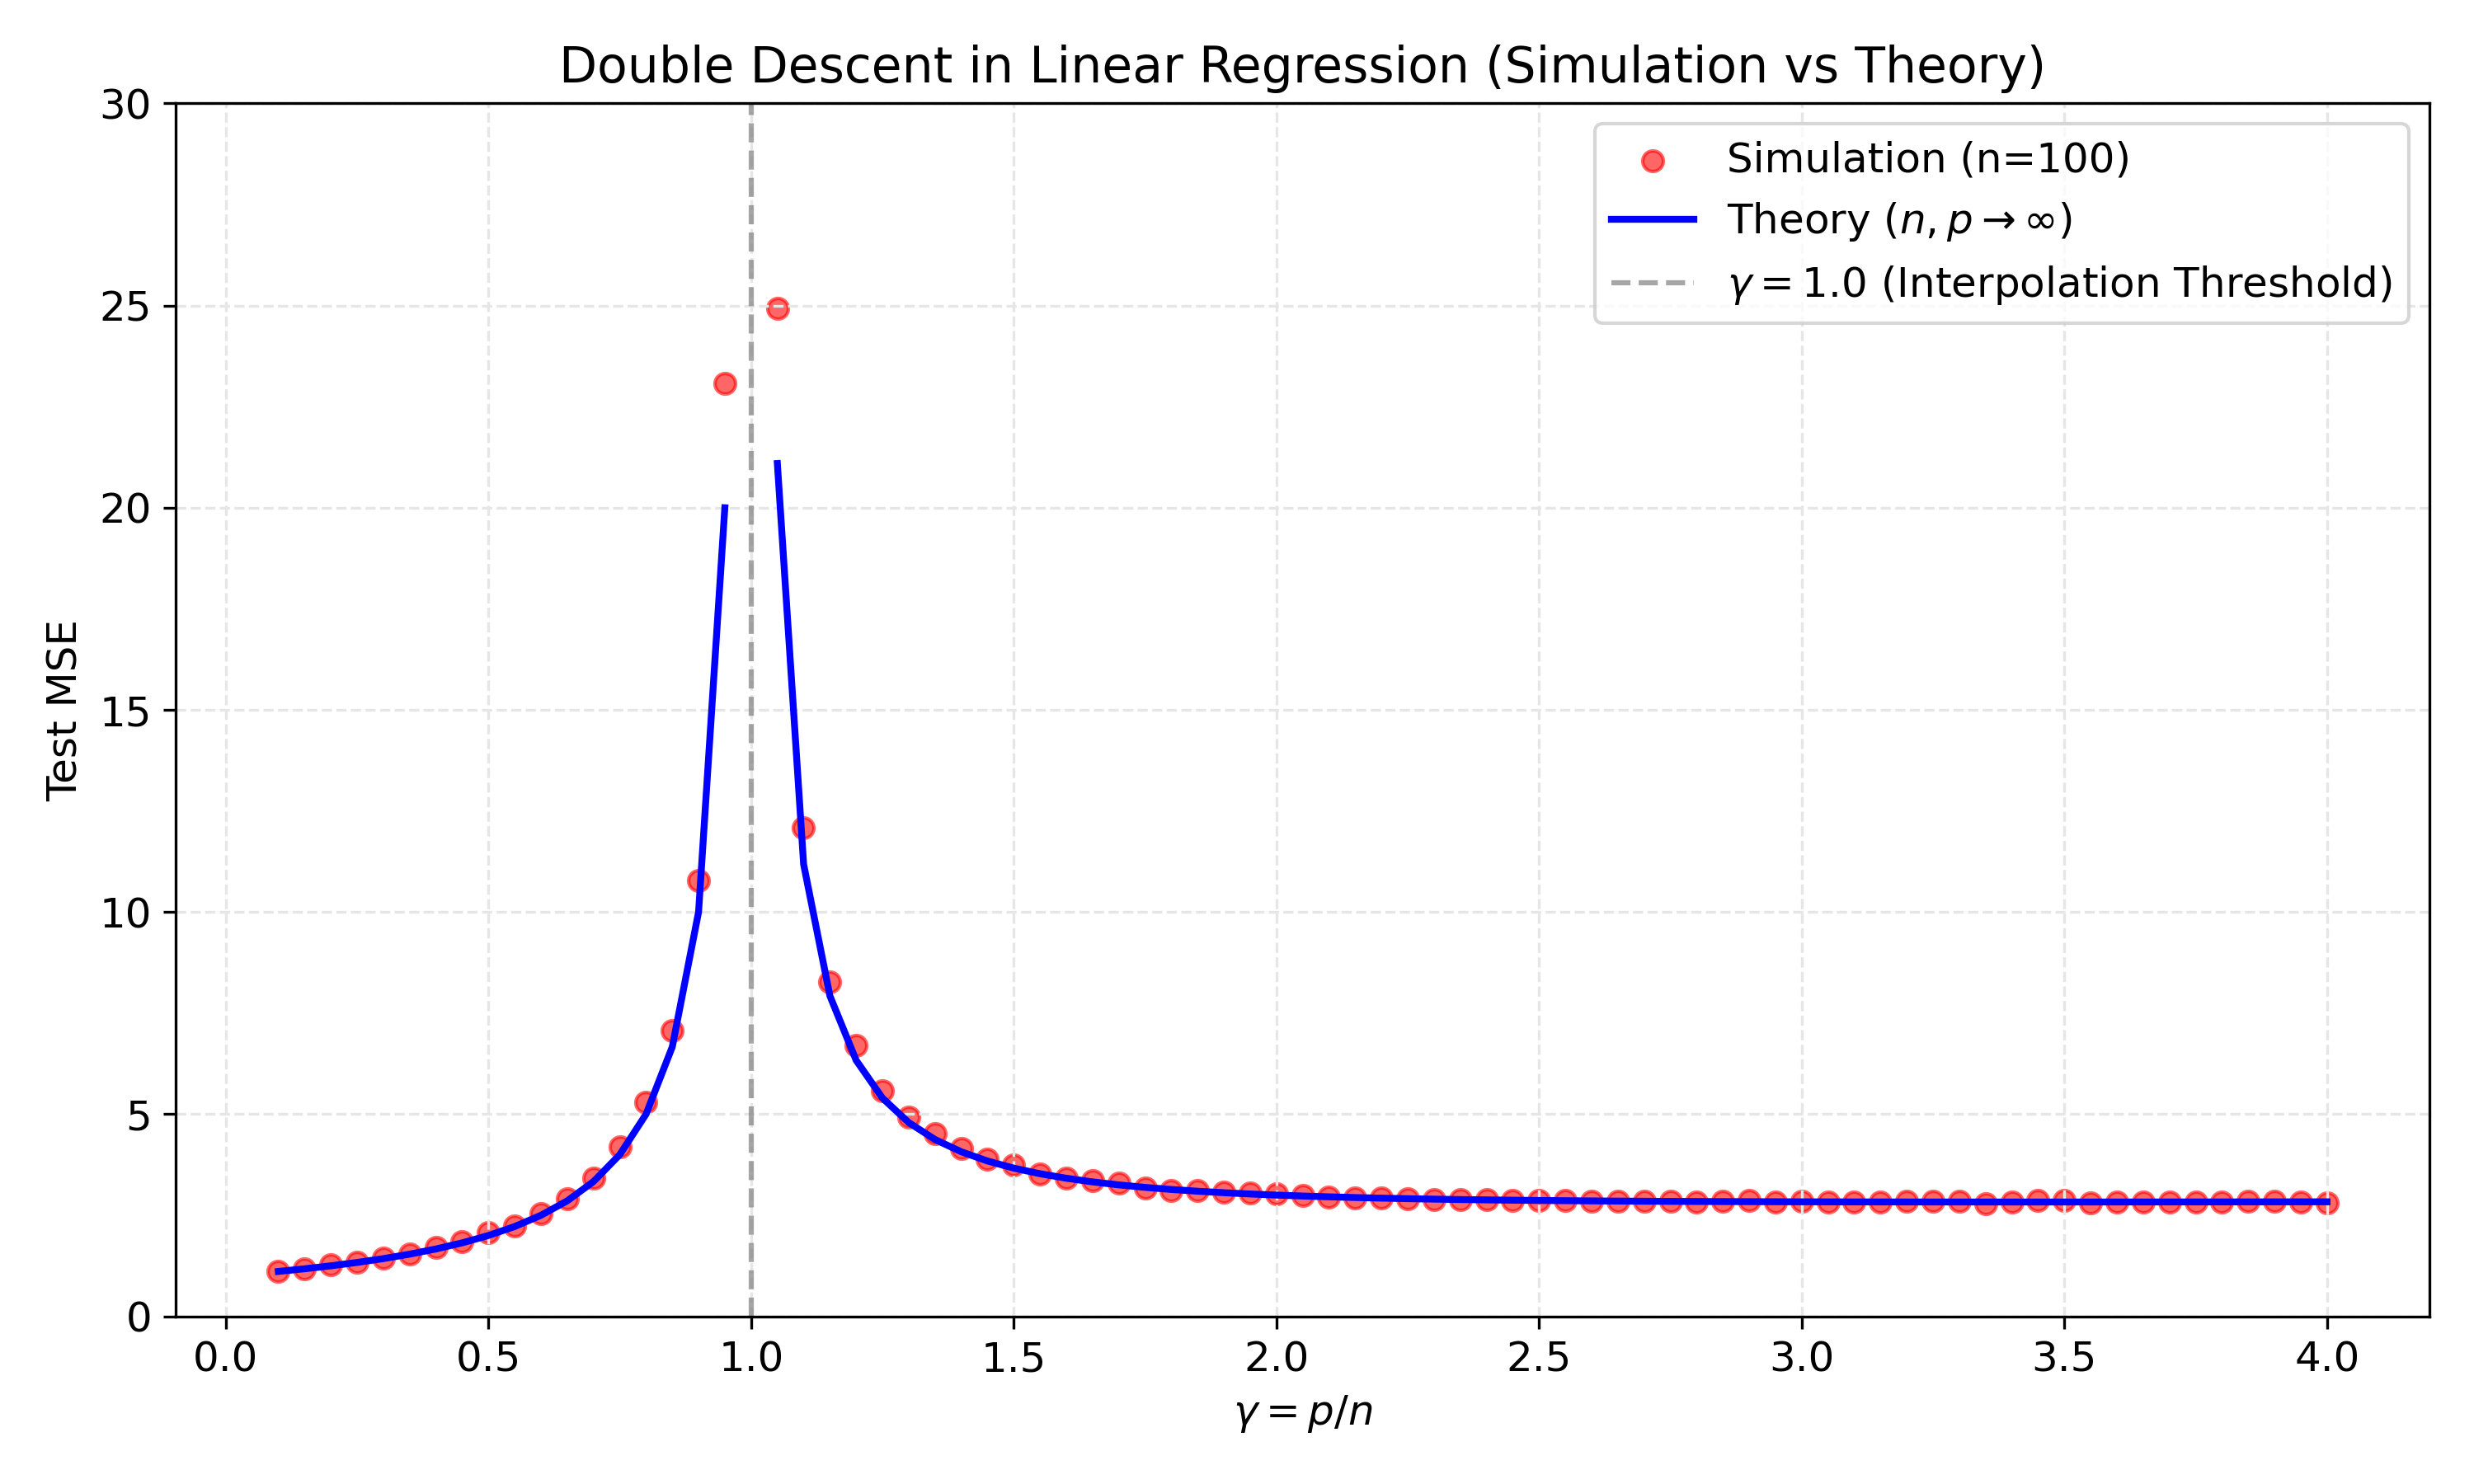
\includegraphics[width=0.7\textwidth]{problem4/plots/double_descent.png}
    \caption{線形回帰における二重降下現象のシミュレーションと理論曲線}
    \label{fig:double_descent}
\end{figure}

$\gamma = p/n \approx 1$ 付近で Test MSE は極大値（発散ピーク）を示すが、過パラメータ領域 $\gamma > 1$ に入ると $\gamma$ の増加にともなって誤差が再び減少する「二重降下現象」が観察される。これは、最小ノルム推定値が暗黙的な正則化（L2ノルム最小化）として機能し、バリアンスの増加を抑え込むためである。
\end{proofbox}

\subsection*{4.5 [難]}
\begin{note}
ランダム行列理論によると $X$ の各成分が独立に $N(0, 1)$ に従うなら、$n, p \to \infty$ において
\begin{equation*}
\begin{cases}
\text{Tr}\left[(X^T X)^{-1}\right] \sim \frac{\gamma}{1-\gamma} & (\gamma < 1 \text{ の時}) \\
\text{Tr}\left[(X X^T)^{-1}\right] \sim \frac{1}{\gamma-1} & (1 < \gamma \text{ の時})
\end{cases}
\end{equation*}
が成立する。\\
また、$X^T (X X^T)^{-1} X$ は $\mathbb{R}^{p \times 1}$ のベクトルを $X$ の行空間 (次元 $n$) へ射影する直交射影行列である。\\
必要なら以上を用いて $\text{Test MSE}$ の理論曲線を導出し、先のプロットに理論曲線を書き足したグラフを作成せよ。
\end{note}
\begin{proofbox}
$n, p \to \infty$（$\gamma = p/n$ 固定）の極限における期待 Test MSE を導出する。

\begin{description}
    \item[1. $\gamma < 1$ の場合 ($n \ge p$)]
    ランダム行列理論より $\text{Tr}\left[(X^T X)^{-1}\right] \sim \frac{\gamma}{1-\gamma}$ を 4.3節の結果に代入すると以下を得る。
    \begin{equation}
    E[\text{Test MSE}] \sim \sigma^2 \left(1 + \frac{\gamma}{1-\gamma}\right) = \frac{\sigma^2}{1-\gamma}
    \end{equation}

    \item[2. $\gamma > 1$ の場合 ($n < p$)]
    バイアス項について、独立な正規乱数からなる $X$ の行空間（次元 $n$）への直交射影行列 $P_X$ は一様にランダムな $n$ 次元部分空間を形成するため、固定された $\bm{\beta}$ の射影の自乗ノルムの期待値は次元の比から次のように得られる。
    \begin{equation}
    E_X \left[ \bm{\beta}^T (I_p - P_X) \bm{\beta} \right] = \|\bm{\beta}\|^2 \frac{p-n}{p} = \|\bm{\beta}\|^2 \left( 1 - \frac{1}{\gamma} \right)
    \end{equation}
    また、バリアンス項は $\text{Tr}\left[(X X^T)^{-1}\right] \sim \frac{1}{\gamma-1}$ より $\frac{\sigma^2}{\gamma-1}$ となる。以上を合わせて次式を得る。
    \begin{equation}
    E[\text{Test MSE}] \sim \sigma^2 + \|\bm{\beta}\|^2 \left( 1 - \frac{1}{\gamma} \right) + \frac{\sigma^2}{\gamma - 1}
    \end{equation}
\end{description}

今回のシミュレーション値（$\sigma^2 = 1$, $\|\bm{\beta}\|^2 = 2$）を代入すると、図\ref{fig:double_descent} に示す通り、シミュレーション結果（赤点）と理論曲線（青線）が極めて良好に一致していることが分かる。
\end{proofbox}


\section*{[生成 AI]}

\subsection*{使用した AI}
\begin{note}
本課題においてどの生成 AI を使用したか、モデルを含めて書け。なぜその AI を選んだか、理由もあれば書くこと。
\end{note}
\begin{proofbox}
本課題では、Google DeepMindの開発した \textbf{Gemini 3.5 Flash} (Medium / Flashモデル) を使用した。このモデルを選択した理由は、マルチファイルコンテキストの処理能力が高く、LaTeXの表組み・図の相対配置コードやPythonの実行スクリプト等の複数ファイルを正確に把握しながら、高速かつ的確な応答が得られるためである。
\end{proofbox}

\subsection*{工夫}
\begin{note}
各問題に対して AI を使った時の会話ログの共有リンクを載せよ。また、その会話で行った工夫や意識した点があれば書け (ex. AI に自分の考えを先に説明した、AI の回答を検証した)。共有リンクを作成すると公開情報になるため、本名や学籍番号などの個人情報は会話に入れないよう注意すること。
\end{note}
\begin{proofbox}
各問題の解答作成時にAIと対話したセッションの会話ログ、および本レポートに付随する理論・数式解説ドキュメントは、個人情報を除外した形でマークダウンファイルとして保存し、以下の一般公開GitHubリポジトリにアップロードした。
\begin{itemize}
    \item リポジトリURL: \href{https://github.com/KokinCho/4S_physics_public/tree/main/\%E6\%A9\%9F\%E6\%A2%B0\%E5%AD\%A6\%E7\%BF%92%E6%A6%82%E8%AB%96}{\texttt{https://github.com/KokinCho/4S\_physics\_public/tree/main/機械学習概論}}
    \item 会話ログファイル: 
    \begin{itemize}
        \item \texttt{conversation\_with\_Gemini\_3\_5\_Flash\_1(Transcribing Machine Learning Exam).md} (問題のLaTeX書き起こしおよび問題1の作成・検証)
        \item \texttt{conversation\_with\_Gemini\_3\_5\_Flash\_2(Analyzing Ensemble Model Variance).md} (問題2の条件付き/周辺分散の検証および課題全体の完成)
    \end{itemize}
    \item 副生成された学習用の数式・理論解説ファイル: 
    \begin{itemize}
        \item \texttt{scratch/problem1\_math\_explanation.md} (L1/L2正則化の幾何学的・代数学的メカニズムとElastic Netの理論的背景)
        \item \texttt{scratch/math\_explanation\_2.md} (決定木・Bagging・Random Forestのバイアス・バリアンス分解と分散低減の数学的証明)
        \item \texttt{scratch/math\_explanation\_3.md} (Baggingにおける予測相関 $\rho$ の実測と決定木不安定性による相関減少の要因分析)
        \item \texttt{scratch/problem2\_variance\_discussion.md} (周辺分散評価におけるBaggingとRandom Forestのプラトー床値の差が小さくなる統計的要因)
        \item \texttt{scratch/conditional\_vs\_marginal\_comparison.md} (条件付き分散と周辺分散のシミュレーション設計における数学的対比)
        \item \texttt{scratch/math\_explanation\_7.md} (課題2.2で検証した3つのサンプリング条件設定の統計学的メカニズム比較表)
        \item \texttt{scratch/math\_explanation\_4.md} (Kullback-Leibler情報量の定義、自由エネルギー差との物理的接続、およびJensenの不等式を用いた非負性証明)
        \item \texttt{scratch/math\_explanation\_5.md} および \texttt{scratch/math\_explanation\_11.md} (線形回帰の推定量期待値・共分散およびTest MSE期待値のWishart極限・ランダム行列理論を用いた漸近導出)
    \end{itemize}
\end{itemize}

AIを利用するにあたり意識した工夫は以下の通り。第一に、丸投げするのではなく「課題プリントのPDFをテキストに起こし、回答用テンプレートを作成する」というように、段階的に指示を与えた。第二に、AIの生成した解答や計算コードをそのまま鵜呑みにせず、実際のシミュレーションの挙動（問題1でL2正則化のパラメータ数が減少しなかった件や、問題2の分散が頭打ちにならない問題など）と照らし合わせ、不整合があれば追加で検証や数理的な対話を行った。第三に、自分自身の学習効率を上げるため、作成するPythonスクリプトには詳細な日本語コメントを付記するよう指示し、数理的証明を別途Markdownで解説させるなどの工夫を凝らした。
\end{proofbox}

\subsection*{感想}
\begin{note}
AI を利用したことで理解が深まった点、逆に AI では解決できなかった点があれば書け。
\end{note}
\begin{proofbox}
\textbf{【理解が深まった点】} \\
二重降下現象における過パラメータ領域の最小ノルム推定量が持つ暗黙的な正則化効果や、ランダム行列理論を用いた期待 Test MSE の漸近的導出など、講義スライドの数式をコードと理論の両面からトレースすることで数学的な理解が大幅に深まった。また、問題2の周辺分散と条件付き分散の数学的違いや、有限サンプルの重複度が木同士の相関に与える影響といった、教科書を読むだけでは見落としがちなシミュレーション設計上の落とし穴についてAIと議論し、検証できたことは非常に有意義だった。

\textbf{【解決できなかった点】} \\
有限データ（$N=395$）における周辺分散の計算時に、元の \texttt{train\_size=0.8} の設定では試行間のデータ重複が大きすぎて Bagging と Random Forest の相関 $\rho$ がどちらも極めて高くなり、グラフ上で両者の挙動（床値の差）がほとんど重なってしまう問題が発生した。この「実験設計と理論の乖離」に対して、AIは当初それに気付かず、こちらが指摘したことで初めて「データサイズを減らして重複を抑える」追加検証を行うに至った。また、macOSにおけるPython並列処理のプロセス生成オーバーヘッド（\texttt{spawn}方式）による時間ロスなど、ローカルな計算環境の最適化についてはAIだけではスマートに解決できず、ローカル環境のシステム的なデバッグが必要となった。
\end{proofbox}

\begin{thebibliography}{10}
    %(本)著者名. 書名. 出版社, 出版年.
    %(雑誌論文)著者名. 論文名. 誌名. 出版年, 巻数, 号数, p.始め-終わり.
    %(web)著者名. “ページ名”. サイト名. 更新日. 入手先URL, (閲覧日).
    \bibitem[1]{bib1}
\end{thebibliography}

\end{document}